\documentclass[12pt]{scrreprt}

%% Allgemeine Hinweise
% 
% - Windows ben�tigt Pearl zum Kompilieren
% - Guter Editor "TexStudio"
% - Nicht vergessen jedes Tex Dokument auf ISO-8859-1 zu stellen
% - Kompilierreihenfolge:
%		1. Makeglossaries
%		2. Biber
%		3. PdfLaTeX
%		4. Interner PDF-Betrachter

%--------------------------------------------------------------------------
% LaTeX packages
%--------------------------------------------------------------------------
\usepackage[ngerman]{babel}		% Neue Deute Rechtschreibung
\usepackage{pdfpages}	% PDF Import
\usepackage{geometry}	% Seitenformatierung (links, rechts usw..)
\usepackage{url}	% Urls
\usepackage{ae}		% Bessere Fonts unterst�tzung
\usepackage[latin1]{inputenc}	% Lateinisch und wichtig f�r MAC
\usepackage[T1]{fontenc}	% Westeurop�ische Kodierung
\usepackage{lmodern}	% Neue deutsche Trennungsregeln, etc 
\usepackage{mathptmx}	% Schriftart (Times New Roman)
\usepackage{acronym}	% Acronyme
\usepackage[onehalfspacing]{setspace}	% Eineinhalb Zeilen Abstand
\usepackage{titlesec}	% Titel Formatierung
\usepackage{hyperref}	% Klickbare Links
\usepackage{minitoc}	% Mini Inhaltsverzeichnis nach jeder �berschrift
\usepackage[headsepline,footsepline]{scrpage2}	% Kopf und Fu�zeilen (Seitenzahl)
\usepackage{listings}	% Quellcode
\usepackage{color}	% Farben f�rs Listing
\usepackage{float}	% Bilder zentrieren
\usepackage[right]{eurosym}
\usepackage[most]{tcolorbox} % Definitionen
\usepackage[autostyle, german=quotes]{csquotes}
\usepackage[backend=biber, style=alphabetic, citestyle=alphabetic]{biblatex}
\usepackage{chngcntr}
\usepackage{caption}
\usepackage{amsmath}
\usepackage{cleveref} % Definitionen
\usepackage[nonumberlist,	% Keine Seitenzahlen anzeigen
						acronym,	% Ein Abk�rzungsverzeichnis erstellen
						toc,	% Eintr�ge im Inhaltsverzeichnis
						section]	% Im Inhaltsverzeichnis auf section-Ebene erscheinen
						{glossaries}	% Glossar

%-----------------------------------------------------------------------------
% Settings
% ********
% Anmerkung: Die meisten Kommandos wurden in der 07_Settings/Settings.tex
% 						Datei erstellt und sollten auch nur dort ver�ndert werden.
%
%-----------------------------------------------------------------------------
% !TEX root = Settings.tex

%################################################################## COMMANDS
%##################################################################
%################################################################## 

\newcommand{\backsl}{\verb|\|} % Backslash

\newcommand{\secline}{\vspace{-1.2em}	% Linie
	\par\noindent\rule{\textwidth}{0.4pt}} 

\newcommand{\emptysite}{\newpage	% Leere Seite
	\thispagestyle{empty}
	\section*{}}

% Glossarzusatz
\renewcommand{\glossarysection}[2][]{\chapter*{#1}}	

% Farbiger Punkt
\newcommand{\tikzcircle}[2][red,fill=red]{\tikz[baseline=-0.5ex]\draw[#1,radius=#2] (0,0) circle ;}

% Abbildungsverzeichnis
\newcommand{\abbildungsverzeichnis}{\newpage
	\phantomsection
	\addstarredchapter{\textbf{Abbildungsverzeichnis}}
	\listoffigures
}

% Tabellenverzeichnis
\newcommand{\tabellenverzeichnis}{\newpage
	\phantomsection
	\addstarredchapter{\textbf{Tabellenverzeichnis}}
	\listoftables
}

% Acronyme
\newcommand{\abkuerzungen}{
	% !TEX root = Acronym.tex
\newpage
\phantomsection
\addstarredchapter{\textbf{Abk�rzungsverzeichnis}}

\chapter*{\huge\textbf{Abk�rzungsverzeichnis}}
\begin{acronym}[Bash]
	\acro{BDD}{Behavior Driven Development}
	\acro{GUI}{Graphical User Interface}
	\acro{HTML}{Hypertext Markup Language}
	\acro{IDE}{Integrated Development Environment}
	\acro{QA}{Quality Assurance}
	\acro{QM}{Qualit�tsmanagement}	
\end{acronym}
}

% Glossar
\newcommand{\glossar}{
	\newpage
	\phantomsection	
	\addstarredchapter{\textbf{Glossar}} % F�gt "Glossar" zum Inhaltsverzeichnis hinzu		
	%\addcontentsline{toc}{chapter}{\textbf{Glossar}}	% F�gt "Glossar" zum Inhaltsverzeichnis hinzu
	\printglossary[style=altlist,title=Glossar]		% Glossar
	\newpage
}

% Heading Style setzen
\newcommand{\headstyle}{
	\pagestyle{scrheadings}	% Style
	\clearscrheadfoot
	\ofoot[\pagemark]{\pagemark}
	\ohead{\headmark}
	\automark[]{chapter}
	\setheadsepline{1pt}
	\setfootsepline{0pt}
}

% Heading Style setzen (Seitenzahl Rechts)
\newcommand{\headstyleright}{
	\pagestyle{scrheadings}	% Style
	\cfoot[]{}	% [plain-Seiten]{normale Seiten} 
	\ofoot[\pagemark]{\pagemark}	% Seitenzahl
	\setheadsepline{0pt}
	\setfootsepline{0pt}
}

\newcommand{\inhaltsverzeichnis}{
	\cleardoublepage\pdfbookmark{\contentsname}{toc}
	\tableofcontents
	\clearpage
	\newpage
}

\newcommand{\literaturverzeichnis}{
	\phantomsection
	\addcontentsline{toc}{chapter}{Literatur}	% �berschrift
	\printbibliography	
}

\newcommand{\anhangstart}{
	\newpage
	%\pagenumbering{arabic}	% Arabische Ziffern
	
	\renewcommand\appendix{\par 
		\setcounter{section}{0}% 
		\setcounter{subsection}{0}% 
		\setcounter{figure}{0}% 
		
		\renewcommand\thesection{\Alph{section}}% 
		\renewcommand\thefigure{\Alph{section}\arabic{figure}}} 
	
	\numberwithin{table}{section} 
	\numberwithin{figure}{section} 
	
	
	\appendix 
	\pagestyle{empty}
	\captionsetup{listof=false}
}

\newcommand{\roemischenummerierung}{
	\pagenumbering{Roman}
}

\newcommand{\arabischenummerierung}{
	\pagenumbering{arabic}
}

%################################################################## OTHER
%##################################################################
%################################################################## 

\titleformat{name=\chapter,numberless}[display]{\normalfont\huge\bfseries}{\titlerule}{-6,9ex}{}[\vspace{3ex}]
\titlespacing{name=\chapter,numberless}{0em}{1.0em}{0em}
\titleformat{\chapter}{\normalfont\huge\bfseries}{\thechapter}{18pt}{\Huge}[{\vspace{0,6ex}\titlerule[0.8pt]\vspace{3ex}}]
\titlespacing{\chapter}{0em}{-4.0em}{0em} % {left}{before}{after}[right]
\titleformat{\section}{\normalfont\LARGE\bfseries}{\thesection}{16pt}{\LARGE}
\titleformat{\subsection}{\normalfont\Large\bfseries}{\thesubsection}{14pt}{\Large}
\titleformat{\subsubsection}{\normalfont\large\bfseries}{\thesubsubsection}{14pt}{\large}

\addbibresource{04_Literatur/Literatur.bib}
\AtBeginDocument{\counterwithin{lstlisting}{section}}
\geometry{a4paper, left=30mm, right=25mm, bottom=25mm, top=25mm}	% Text Formatierung
% !TEX root = Glossar.tex
\makeglossaries

\newglossaryentry{venturecapital}{ 
	name=Venture-Capital, 
	description={ 
		Unter Venture Capital versteht man die Finanzierung eines nicht b�rsennotierten Unternehmens mit Eigenkapital. Dabei wird das Unternehmen in der Regel zum Zeitpunkt der Beteiligung privat gehalten. Entscheidend ist, dass das Eigentum am Unternehmen w�hrend der meisten Zeit der Beteiligung in privaten H�nden liegt \autocite{venture_capital}} 
}

\newglossaryentry{servantleader}{ 
	name=Servant Leader, 
	description={ 
		Ein Servant Leader liebt Menschen und m�chte ihnen helfen. Die Aufgabe eines Servant Leaders ist es daher, die Bed�rfnisse anderer zu ermitteln und zu versuchen, diese Bed�rfnisse zu befriedigen \autocite{servant_leadership}} 
} 

\newglossaryentry{iteration}{ 
	name=Iteration, 
	description={ 
		Eine Iteration ist eine wiederholte Durchf�hrung eines Vorgangs. Die Anzahl der Durchf�hrungen (Iterationen) steht entweder vorher fest oder richtet sich nach der Erf�llung eines Abbruchkriteriums \autocite{definition_iteration} 
	}
} 

\newglossaryentry{stakeholder}{ 
	name=Stakeholder, 
	description={ 
		Anspruchsgruppen sind alle internen und externen Personengruppen, die von den unternehmerischen T�tigkeiten gegenw�rtig oder in Zukunft direkt oder indirekt betroffen sind. Gem�� Stakeholder-Ansatz wird ihnen - zus�tzlich zu den Eigent�mern (Shareholders) - das Recht zugesprochen, ihre Interessen gegen�ber der Unternehmung geltend zu machen \autocite{definition_stakeholder}
	}
}

\newglossaryentry{trialanderror}{ 
	name=Trial and Error, 
	description={ 
		Trial and Error beschreibt einen Weg, ein Ziel zu erreichen oder ein Problem zu l�sen, indem verschiedene Methoden ausprobiert und aus Fehlern gelernt wird \autocite{definition_trialanderror}
	}
}

\newglossaryentry{governance}{ 
	name=Governance, 
	description={ 
		Die Art und Weise, wie in einem Land die Angelegenheiten der Allgemeinheit verwaltet und geregelt werden. \enquote{Governance} ist nicht \enquote{Government} gleich \enquote{Regierung}, sondern umfassender und offener \autocite{definition_governance}
	}
}

\newglossaryentry{workaround}{ 
	name=Workaround, 
	description={ 
		Ein workaround beschreibt eine M�glichkeit, ein Problem zu l�sen, oder etwas trotz des Problems zum laufen zu bekommen, ohne es vollst�ndig zu l�sen \autocite{definition_workaround}
	}
}

\newglossaryentry{coredeliverable}{ 
	name=Core Deliverable, 
	description={ 
		Ein Core Deliverable ist das zentrale Produkt oder Dienstleistung, welches einem Kunden zu Verf�gung gestellt wird \autocite{definition_deliverable}
	}
}

\newglossaryentry{cicd}{ 
	name=Continous Integration, 
	description={ 
		Continous Integration beschreibt einen Softwareentwicklungsprozess, bei dem Teammitglieder h�ufig ihre Arbeit integrieren. Bei jeder Integration wird der Stand automatisch �berpr�ft, um Integrationsfehler so schnell wie m�glich zu erkennen \autocite{definition_ci}
	}
}

\newglossaryentry{devops}{ 
	name=DevOps, 
	description={ 
		Der Begriff besteht aus Development (Dev), der den Softwareentwickler beschreibt, und Operations (Ops), was den IT-Betrieb darstellt. Aus der Kombination beider soll ein Prozessverbesserungsansatz f�r die Bereiche Softwareentwicklung und Systemadministration entstehen. Es wird eine effektivere und effizientere Zusammenarbeit der verschiedenen Bereiche angestrebt \autocite{definition_devops}
	}
}
	% Glossar IMPORT
\setlength{\parindent}{0pt}	% Keine Einr�ckung am Anfang eines Absatzes
\setcounter{biburllcpenalty}{7000}
\setcounter{biburlucpenalty}{8000}

%################################################################## LISTINGS
%##################################################################
%################################################################## 

\renewcommand{\lstlistingname}{Codebeispiel}% Listing -> Codebeispiel
\renewcommand{\lstlistlistingname}{Codeverzeichnis}% List of Listings -> Codeverzeichnis

% Default fixed font does not support bold face
\DeclareFixedFont{\ttb}{T1}{txtt}{bx}{n}{12} % for bold
\DeclareFixedFont{\ttm}{T1}{txtt}{m}{n}{12}  % for normal

% Custom colors
\definecolor{deepblue}{rgb}{0,0,0.5}
\definecolor{deepred}{rgb}{0.6,0,0}
\definecolor{deepgreen}{rgb}{0,0.5,0}
\definecolor{superlightgray}{rgb}{0.97,0.97,0.97}

% Java Style
\lstdefinestyle{java}{
	language=Java,
	basicstyle=\ttm,
	otherkeywords={this},
	breaklines=true,
	tabsize=2,
	keywordstyle=\ttb\color{deepblue},
	emph={MyClass,__init__},          % Custom highlighting
	emphstyle=\ttb\color{deepred},    % Custom highlighting style
	stringstyle=\color{deepgreen},
	frame=tb,                         % Any extra options here
	belowskip=3em,
	belowcaptionskip=1em,
	aboveskip=2em,
	abovecaptionskip=1em,
	captionpos=b,
	showstringspaces=false 
}

% Java Script Style
\lstdefinestyle{travis}{
	language=bash,
	numbers=left,
	stepnumber=5,
	firstnumber=1,
	tabsize=2,
	basicstyle=\ttm,
	breaklines=true,
	alsoletter={:},
	keywords={language:, node_js:, cache:, install:, before_script:, script:},
	keywordstyle=\ttb\color{orange},
	emph={MyClass,__init__},          % Custom highlighting
	emphstyle=\ttb\color{deepred},    % Custom highlighting style
	stringstyle=\color{deepgreen},
	frame=single,                         % Any extra options here
	backgroundcolor=\color{superlightgray},
	ndkeywords={directories:},
	ndkeywordstyle=\ttb\color{deepblue},
	belowskip=2em,
	aboveskip=2em,
	abovecaptionskip=1em,
	captionpos=b,
	showstringspaces=false 
}

% Java Script Style
\lstdefinestyle{cypress}{
	language=Java,
	numbers=left,
	stepnumber=5,
	firstnumber=1,
	tabsize=2,
	basicstyle=\ttm,
	breaklines=true,
	keywords={describe, before, beforeEach, context, it, expect, equal, cy, def},
	keywordstyle=\ttb\color{orange},
	emph={MyClass,__init__},          % Custom highlighting
	emphstyle=\ttb\color{deepred},    % Custom highlighting style
	stringstyle=\color{deepgreen},
	frame=single,                         % Any extra options here
	backgroundcolor=\color{superlightgray},
	ndkeywords={assert, break, case, catch, continue, debugger, default, delete, do, else, false, finally, for, function, if, in, instanceof, new, null, return, switch, this, throw, true, try, typeof, var, void, while, with},
	ndkeywordstyle=\ttb\color{deepblue},
	belowskip=2em,
	aboveskip=2em,
	abovecaptionskip=1em,
	captionpos=b,
	showstringspaces=false 
}

% Python Style
\lstdefinestyle{python}{
	language=python,
	numbers=left,
	basicstyle=\ttm,
	otherkeywords={self},
	keywordstyle=\ttb\color{deepblue},
	emph={MyClass,__init__},          % Custom highlighting
	emphstyle=\ttb\color{deepred},    % Custom highlighting style
	stringstyle=\color{deepgreen},
	frame=tb,                         % Any extra options here
	belowskip=3em,
	aboveskip=2em,
	abovecaptionskip=1em,
	captionpos=b,
	showstringspaces=false  
}

% Bash Style
\lstdefinestyle{bash}{
	language=bash,
	basicstyle=\ttm,
	numbers=left,
	stepnumber=5,
	firstnumber=1,
	backgroundcolor=\color{superlightgray},
	otherkeywords={},
	keywordstyle=\ttb\color{deepblue},
	emph={\$},          % Custom highlighting
	emphstyle=\ttb\color{deepred},    % Custom highlighting style
	stringstyle=\color{deepgreen},
	frame=single,                         % Any extra options here
	showstringspaces=false,
	belowskip=2em,
	aboveskip=2em,
	abovecaptionskip=1em,
	captionpos=b
}

%################################################################## DEFINITONS
%##################################################################
%################################################################## 

\newtcbtheorem[number within=chapter]{Definition}{}{
	enhanced,
	attach boxed title to top left={
		xshift=-1mm,
		yshift=-5mm,
		yshifttext=-1mm
	},
	breakable,
	top=0.5em,
	bottom=-0.5em,
	colback=white,
	colframe=black,
	fonttitle=\bfseries,
	boxed title style={
		size=small,
		colback=black,
		colframe=black,
	} 
}{def}

\newenvironment{definition}[2]{ \begin{Definition}[adjusted title=#1]{}{#2} 
		\textbf{} }{\end{Definition}}

%-----------------------------------------------------------------------------
% START OF DOCUMENT														---------------------
%-----------------------------------------------------------------------------
\begin{document}

% Deckblatt & Einverst�ndnisserkl�rung

\includepdf[pages={1}]{03_PDFs/Deckblatt.pdf}
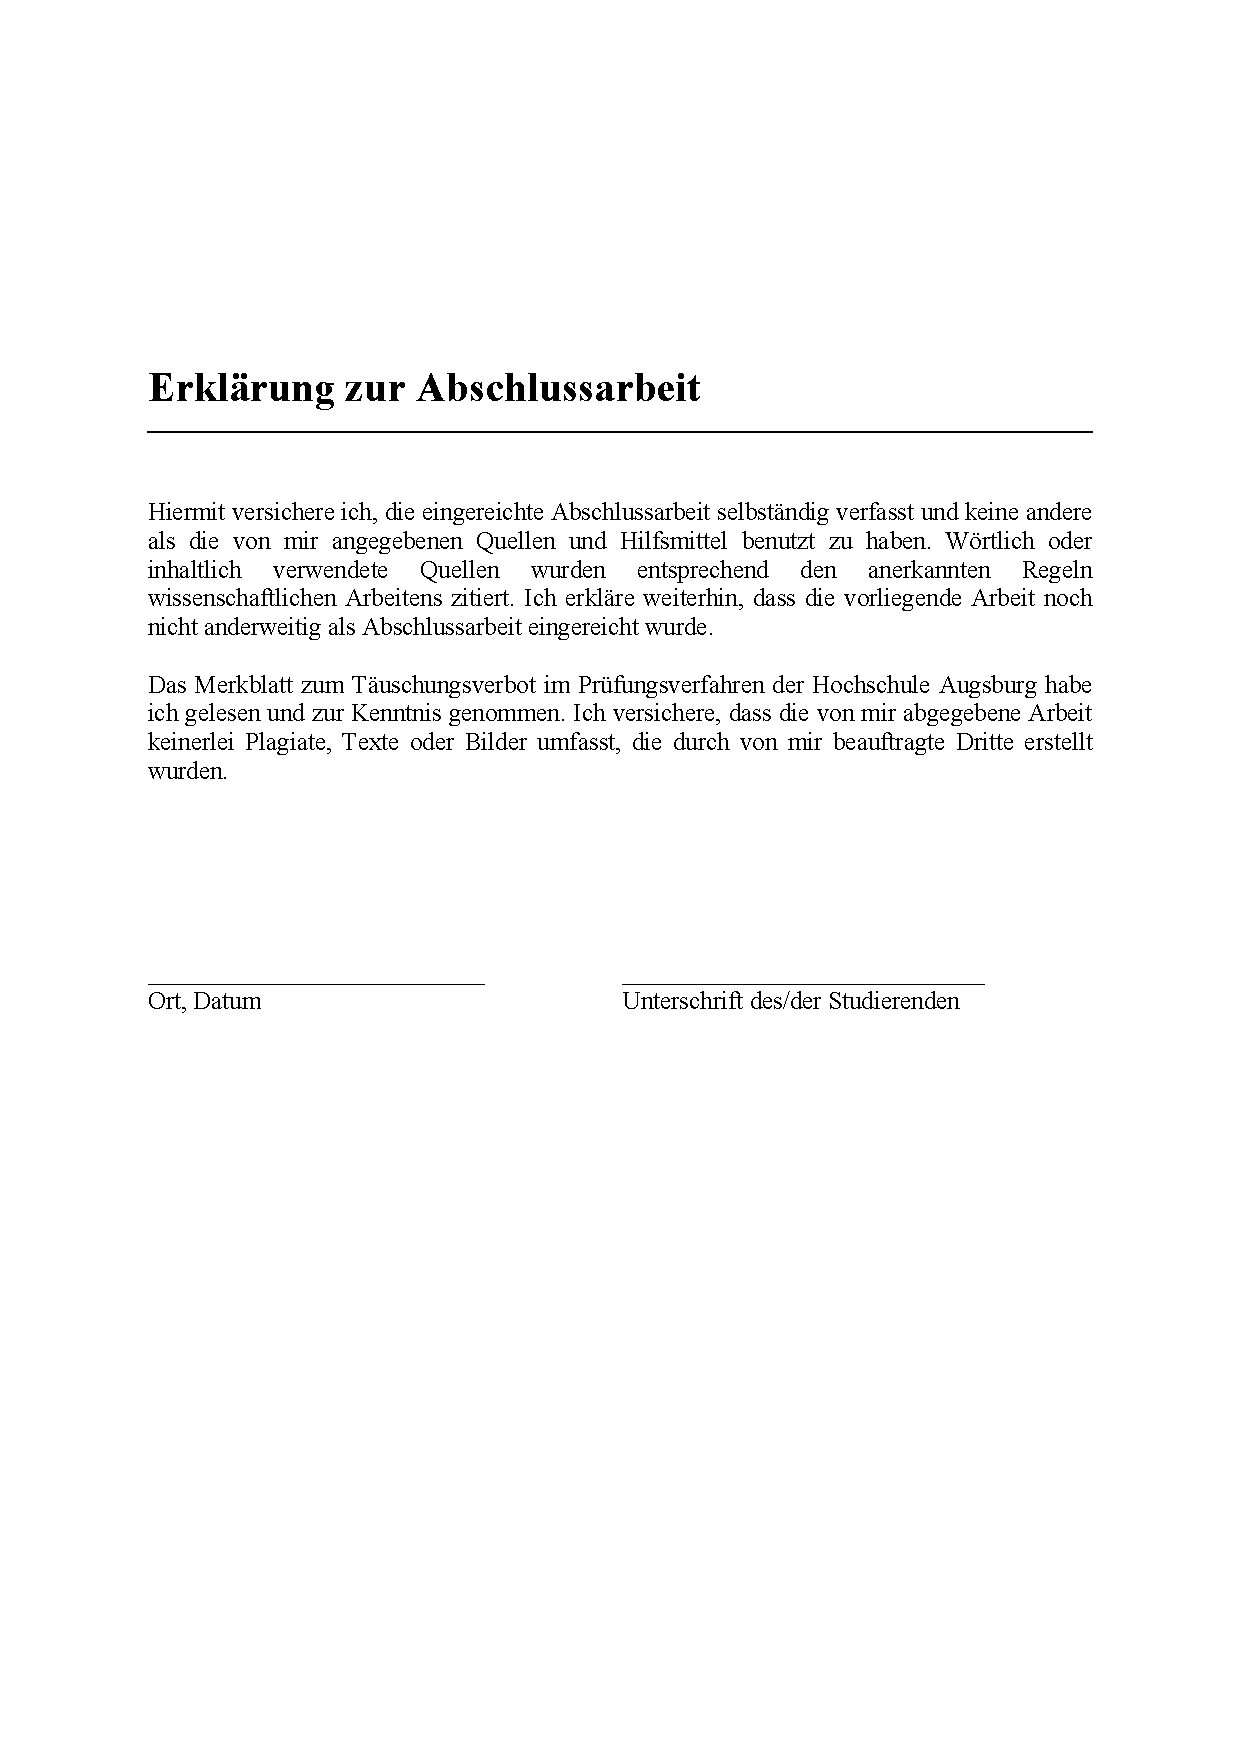
\includepdf[]{03_PDFs/Erstellungserklaerung.pdf}

% Seitenzahlformatierung (rechts)
\headstyleright

% R�mische Ziffern
\roemischenummerierung

% Setze Seitenzahl
\setcounter{page}{3}	

% Danksagung
% !TEX root = Danksagung.tex

\section*{\huge\textbf{Danksagung}}
\secline
\\\\
HIER DANKSAGUNG

\newpage


% Kurzfassung
% !TEX root = Kurzfassung.tex

\section*{\huge\textbf{Kurzfassung}}
\secline
\\\\
Viele Unternehmen sind derzeit im Umbruch in Richtung Agilit�t, obwohl diese oft die Bedeutung noch nicht genau verstehen. Agilit�t wird von einigen geliebt, von anderen nicht verstanden und vom Rest kategorisch abgelehnt. Eine Studie hat gezeigt, dass agiles Arbeiten nicht nur das Teamklima verbessert, sondern Mitarbeiter auch visions-, aufgabenorientierter und innovationsfreudiger arbeiten. Ziel dieser Arbeit ist es, herauszufinden, was genau Unternehmen davon abh�lt, von einer klassischen auf eine agile Arbeitsweise umzusteigen. Um spezifischere Ergebnisse zu erhalten, wurden diese in die drei Arten, Start-up, Mittelstand und Konzern aufgeteilt. Anschlie�end wurde ein Fragebogen erarbeitet, der das Ziel hat, Herausforderungen und Metadaten f�r die jeweiligen Unternehmensarten zu ermitteln. Neben den Ergebnissen der Frageb�gen wurden mithilfe von Erfahrungsberichten und Interviews weitere Daten erhoben. Um aus den Daten, relevante Informationen herauszufiltern, wurde die qualitative Inhaltsanalyse nach Mayring angewendet. Diese hat 45 Herausforderungen und einige Metadaten zutage gebracht. Alle Herausforderungen wurden anschlie�end aus der Sicht jeder Unternehmensart mithilfe der Metadaten bewertet. Die Bewertung hat gezeigt, dass die gr��ten Herausforderungen f�r Start-ups in der Abh�ngigkeit zu den Investoren liegen. Der Mittelstand im Vergleich ist h�ufig traditionell gepr�gt, was Herausforderungen in der Unternehmenskultur und der Verkn�pfung von IT-Systemen mit sich bringt. Dagegen liegen die Herausforderungen von Konzernen, verursacht durch die oft durchwachsene Unternehmensstruktur, oft in der Komplexit�t, der Dauer der Transformation und der damit einhergehenden hohen Kosten. Trotz der Herausforderungen muss jedes Unternehmen f�r sich entscheiden, ob es den langen Weg einer Transformation gehen m�chte. 

\newpage


% Inhaltsverzeichnis
\inhaltsverzeichnis

% Kopf und Fu�zeile
\headstyle

% Abbildungsverzeichnis
\abbildungsverzeichnis

% Tabellenverzeichnis
\tabellenverzeichnis

% Acronyme
\abkuerzungen

% Glossar
\glossar

% Arabische Ziffern
\arabischenummerierung


%-----------------------------------------------------------------------------
% HAUPTARBEIT																	HAUPTARBEIT
%-----------------------------------------------------------------------------
% !TEX root = Einleitung.tex

\chapter{Einleitung}

Jedes Projekt mit dem Ziel Software zu entwickeln, ist individuell. Aus diesem Grund gibt es in den seltensten F�llen wiederholbare Prozesse. Reproduzierbare Prozesse k�nnen durch klare Anweisungen mithilfe anschlie�ender Kontrolle befehligt oder gesteuert werden. Kreative Prozesse hingegen scheitern bei diesem Ansatz, da diese individuell, je nach Situation gesteuert werden m�ssen \autocite[vgl.][]{agiles_projektmanagement}. Um genau diese Art von Steuerung erreichen zu k�nnen, versuchen immer mehr Unternehmen einen agilen Ansatz. Diese Vorgehensweise hat das Ziel, eine kreative Probleml�sung im Team zu f�rdern, da sich Kreativit�t nicht einfach anordnen l�sst \autocite[vgl.][S.VII]{agiler_fuehren}.
\\
\begin{definition}{Definition Agile F�hrung (Quelle: \autocite{agiler_fuehren})}{def:agile_fuehrung}
	\\ 
	Agile F�hrung unterst�tzt Mitarbeiter dabei, schnell und kreativ auf wechselnde Bed�rfnisse von Kunden und M�rkten zu reagieren. Sie ist ein Mindset, eine Haltung. Sie nutzt eine offene Toolbox mit Coachingwerkzeugen, die die Zusammenarbeit verbessern, sowie Methoden zur Reduktion von Komplexit�t.
	\\
\end{definition}

Unternehmens- und F�hrungskulturen sind derzeit in vielen Unternehmen im Umbruch in Richtung Agilit�t. Bei all den Ver�nderungen in diese Richtung wissen viele Unternehmen noch nicht, was es genau bedeutet, als Unternehmen, Team oder F�hrungskraft agiler zu werden. Eine Studie (siehe \autocite[vgl.][VII]{agiler_fuehren}) mit dem Namen \enquote{Teamklima f�r Innovation} wollte herausfinden, ob sich das Teamklima in nicht-agilen Gruppen von den agilen unterscheidet. Das Ergebnis hat gezeigt, dass nicht nur das Teamklima innerhalb agil arbeitender Teams besser war, sondern diese auch visions-, aufgabenorientierter und innovationsfreudiger agieren. Zudem verbessern agile Elemente wie Visualisierung, Teamentscheidung, Retrospektive, iterative Planung und Stand-up-Meetings die Zusammenarbeit \autocite[vgl.][S.VII-VIII]{agiler_fuehren}.
\\\\ 
Das Wort \enquote{Agil} ist eine Art Reizwort, das von einigen geliebt, von anderen nicht verstanden und vom Rest kategorisch abgelehnt wird. So schrieb die amerikanische Zeitschrift \enquote{Forbes!} (siehe \autocite{managers_hate_agile}), dass Manager \enquote{agile} (Agilit�t) hassen. Die Begr�ndung der Zeitschrift f�r die Abwehrhaltung der Manager lag in einem m�glichen Machtverlust, da Agilit�t im Management gerne mit dem Abbau von F�hrung verwechselt wird. Dabei geht es gar nicht um den strikten Abbau von F�hrung, sondern eher um das F�rdern von flacheren Hierarchien. H�ufig wird die Agilit�t abgelehnt, ohne genau zu wissen, was sich dahinter verbirgt. Diejenigen, die nur eine grobe Idee davon haben, begr�nden ihre ablehnende Haltung mit dem Argument, \enquote{alle machen, was sie wollen} und bef�rchten, dass das konzernweite Chaos ausbricht \autocite[vgl.][S.1]{agiler_fuehren}.
\\\\
Hinsichtlich der Ergebnisse der eben erw�hnten Studie (siehe \autocite[vgl.][VII]{agiler_fuehren} - Teamklima f�r Innovation) stellt sich nun die Frage, ob es nicht genau diese Eigenschaften sind, die ein \enquote{modernes} Projektmanagement in Zeiten, in denen Individualit�t so eine gro�e Rolle spielt, dabei helfen, scheitern zu verhindern. Wenn Agilit�t das Mittel ist, das die Eigenschaften liefert, die ben�tigt werden, um kreative Prozesse zu f�rdern, wieso wenden nicht alle Unternehmen agile Methodiken an? 

\section{Zielsetzung \& Hypothesenbildung} \label{Kap:Zielsetzung}
Ziel dieser Arbeit ist es, herauszufinden, welche Herausforderungen Unternehmen davon abhalten, agile Methodiken anzuwenden. Dabei stellen sich die Fragen, treffen diese Herausforderungen auf alle Unternehmensarten gleicherma�en zu und k�nnen sie �berhaupt bew�ltigt werden? Zus�tzlich zu diesen Fragen werden die folgenden Hypothesen gebildet und im sp�teren Verlauf �berpr�ft:

\begin{itemize}
	\item \textbf{Die Gr��e des Unternehmens spielt eine Rolle}\\
	Desto kleiner ein Unternehmen ist, desto leichter f�llt die agile Transformation.
	
	\item \textbf{Gr��erer Innovationsdruck bei Konzernen}\\
	Je gr��er ein Konzern ist, desto mehr Innovationsdruck hin zu agilen Prozessen ist vorhanden.
	
	\item \textbf{Kosten der agilen Transformation}\\
	Die Kosten der agilen Transformation in Unternehmen, �bersteigen den Wert des Nutzen.
	
	\item \textbf{Unternehmensweites Chaos dank anarchischer Ans�tze}\\
	Bei der Einf�hrung von agilen Prozessen bricht das unternehmensweite Chaos aus.
\end{itemize}

Um die Fragen zu beantworten und die Hypothesen zu �berpr�fen, werden anhand verschiedenster Berichte, eines Fragebogens und darauf basierenden Interviews, Herausforderungen ermittelt. Zus�tzlich zu diesen, sollen auch Metadaten f�r die verschiedenen Unternehmensarten wie etwa Start-up, Mittelstand und Konzern bestimmt werden. Das hilft dabei, Herausforderungen aus der Sicht jeder Unternehmensart zu bewerten. Nach der Bewertung wird zus�tzlich dargelegt, wie die schwerwiegendsten Herausforderungen bew�ltigt werden k�nnen. Um zun�chst zu verstehen, was �berhaupt das Wort \enquote{Agilit�t} bedeutet, wird im n�chsten Kapitel Grundlagen genauer darauf eingegangen. 



% !TEX root = StandDerTechnik.tex

\chapter{Stand der Technik}

Im Folgenden wird beschrieben was Qualit�tsmanagement ist, welche die momentan wichtigsten Testarten sind und von welchen Frameworks Selenium profitiert. Zus�tzlich werden weitere Blickwinkel zu diesem Themengebiet reflektiert und ein �berblick �ber den bisherigen Stand der Forschung gegeben.  

\section{Bedeutung-Qualit�tsmanagement}\label{def:Bedeutung}

\begin{definition}{Definition Qualit�tsmanagement nach DIN-EN-ISO-9000:2000}{def:Definition}
	\\ Aufeinander abgestimmte T�tigkeiten zum Leiten und Lenken einer Organisation bez�glich Qualit�t. \autocite{schwarze2003kundenorientiertes}\\
\end{definition}

Somit beschreibt der Begriff Qualit�tsmanagement alle Ma�nahmen und T�tigkeiten, die notwendig sind, um Qualit�t zu erzeugen \autocite{kochendorfer2004bau}. Qualit�tsmanagement findet unternehmensweit statt und erfordert daher eine sehr gute Koordination. \autocite{reinhart1996unternehmensstrategie}.

\subsection{Qualit�tsmanagementsysteme}
Damit Qualit�tsmanagement �berhaupt umgesetzt werden kann, wird ein sogenanntes Qualit�tsmanagementsystem ben�tigt. Es enth�lt die Aufbau- und Ablauforganisation, um alle Qualit�tsmanagementaufgaben durchzuf�hren und die folgenden Fragen zu kl�ren \autocite{kochendorfer2004bau}:

\begin{itemize}
	\item \textbf{Was?}		- Um welche qualit�tsbezogenen Aufgaben handelt es sich?
	\item \textbf{Wer?} 	- Welche Personen nehmen qualit�sbezogene Aufgaben wahr?
	\item \textbf{Wann?}	- Wie gestaltet sich der Ablauf qualit�tsbezogener Aufgaben?
	\item \textbf{Wie?}		- Was f�r Verfahren werden angewendet?
\end{itemize}

Mit der Norm DIN-EN-ISO-9000 wurde ein einheitlicher Standard zum Vergleich und Aufbau verschiedener Qualit�tsmanagementsysteme erstellt \autocite{kochendorfer2004bau}.

\subsection{Qualit�t}
Der Begriff \enquote{Qualit�t} sagt aus, dass jeder Kunde, W�nsche aufgrund der von ihm festgelegten Anspr�che besitzt, die gegen�ber dem Hersteller gerne als Qualit�tsanforderungen oder in Form von Erwartungen ge�u�ert werden. Durch diese Anforderungen und Erwartungen bildet sich wiederum eine Vorstellung des Produktpreises. Was f�r eine Qualit�t ein Produkt besitzt, ergibt sich schlie�lich erst durch den Vergleich zwischen der Beschaffenheit und den Produktanforderungen des Kunden \autocite{qualitaetsmanagement}.

\section{\acs{QA}-Abteilung}\label{def:qaAbteilung}
Eine Quality Assurance (\acs{QA})-Abteilung besch�ftigt sich mit der Sicherstellung vorher definierter Qualit�tsanforderungen. Gro�teils geht es darum, die technische Zuverl�ssigkeit von Prozessen und Produkten eines Unternehmens zu gew�hrleisten. Diese Gew�hrleistung f�hrt zu einer Risikominimierung f�r das Unternehmen und den Kunden. Ein weiterer Aspekt ist die Kostenreduktion durch eine geringere Haftung auf Schadensersatz gegen den Hersteller. \acs{QA}-Abteilungen m�ssen daher st�ndig die Qualit�t der Produkte und Dienstleistungen im Auge behalten und deren Zuverl�ssigkeit sicherstellen \autocite{qa_buch}.

\section{Testpyramide} \label{def:testpyramide}

\begin{figure}[H]
	\centering
	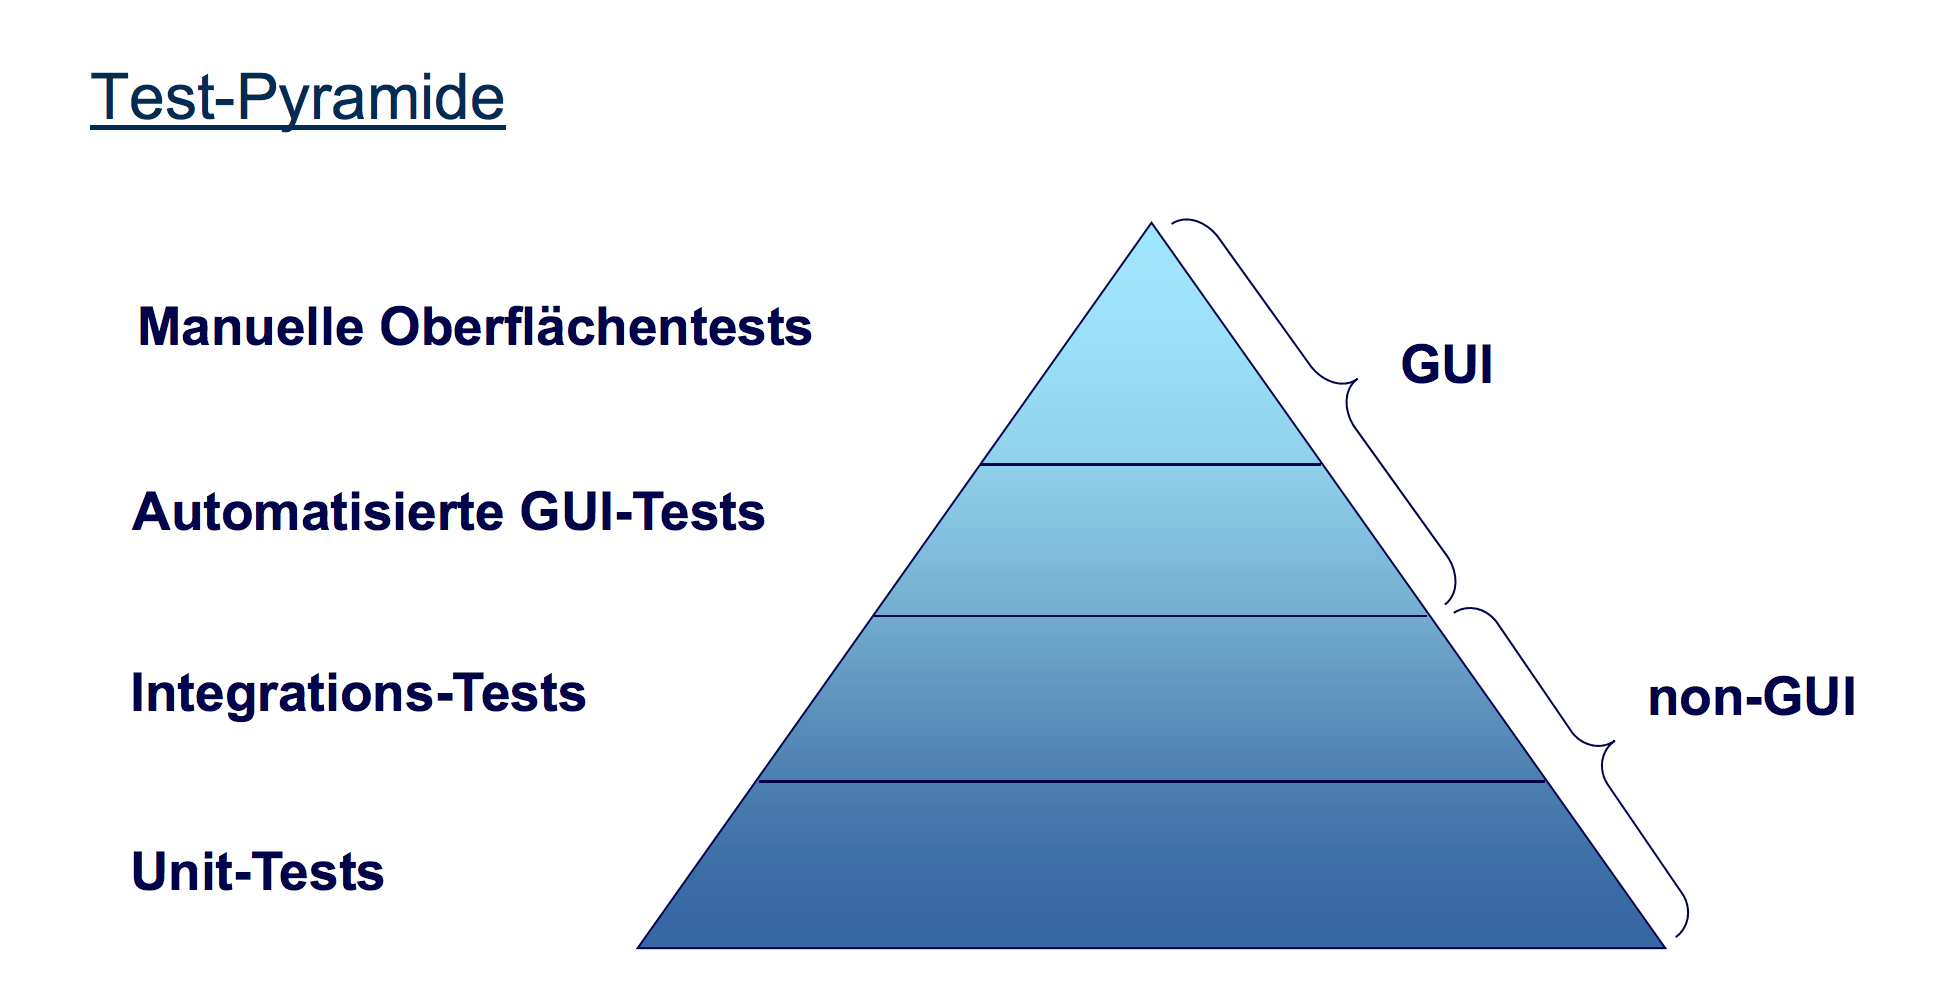
\includegraphics[width=1.0\textwidth]{06_Bilder/testpyramide.png}
	\setlength{\abovecaptionskip}{-1em}
	\caption{Testpyramide nach (Quelle: \autocite{frueheTesterfaengtdenWurm})}
	\label{img:testpyramide}
\end{figure}  

Zur besseren Einordnung bestimmter Tests wurde von Mike Cohn das Konzept der Test-Pyramide entwickelt. Die Pyramide soll die richtige Verteilung der unterschiedlichen Testarten verdeutlichen. Idealerweise gibt es im Fundament einen sehr hohen Anteil an einfach zu wartenden Unittests (siehe Kapitel \ref{def:Unittest}). Integrations-Tests (siehe Kapitel \ref{def:Integrationstest}) haben in der Regel l�ngere Ausf�hrzeiten und sind aufwendiger zu pflegen. Durch diesen Umstand werden Integrations-Tests meist nur zur zielgerichteten Pr�fung von kritischen Schnittstellen eingesetzt. Manuelle und automatisierte Oberfl�chentests (GUI-Tests) bilden die Spitze. Diese Tests eignen sich dazu, in der Gesamtheit die Funktionalit�t der Software zu gew�hrleisten. Oberfl�chentests eignen sich nicht dazu, alle m�glichen Zweige innerhalb des Quellcodes zu �berpr�fen, daher sollte ihre Anzahl auch minimal gehalten werden \autocite{testpyramide}. 

\section{Test-Arten} \label{def:Testarten}
Im Kapitel \ref{def:testpyramide} Testpyramide wurde beschrieben welche Testarten sich innerhalb der Testpyramide befinden und welchen Anteil diese ausmachen. Anhand der Testpyramide gegliedert, werden in diesem Kapitel einige Testarten genauer beleuchtet.

\subsection{Unittests} \label{def:Unittest}
Unittests, auch Modultests genannt, werden h�ufig seitens der Entwickler durchgef�hrt. Diese Art von Tests testen s�mtliche Teile (Units) einer Software auf Funktionalit�t. Dabei wird als erstes der Ausgangszustand (Soll-Zustand) definiert. Hierbei werden Werte definiert, die die Funktionalit�t einer Unit gew�hrleisten. Anschlie�end wird bei der Ausf�hrung, der resultierende Wert (Ist-Zustand) mit dem vorher definierten verglichen. Stimmen diese nicht �berein, schl�gt der Test fehl \autocite{testarten}.

\subsection{Integrationstests} \label{def:Integrationstest}
Im Vergleich zu den Unittests, bei denen nur einzelne Module getestet werden, wird bei einem Integrationstest das Zusammenspiel der Module getestet. Die Voraussetzung daf�r ist, dass geeignete Testdaten und Schnittstellen technisch zur Verf�gung stehen. Integrationstests werden mit Testdaten (auch synthetische Daten genannt) durchgef�hrt. Wie auch bei anderen Testarten wird eine Liste mit einzelnen Schritten, die jeweils eine Beschreibung und ein erwartetes Ergebnis definieren, im Vorhinein erstellt und abgearbeitet \autocite{testarten}.

\subsection{Oberfl�chentests (GUI-Tests)}
Unter dem Begriff Oberfl�chentests (GUI-Tests) werden alle Tests verstanden, bei denen der Tester versucht mit dem Produkt �ber die grafische Oberfl�che (GUI) zu interagieren. Bei diesen Tests gibt es verschiedene Vorgehensweisen, die in diesem Kapitel beschrieben werden.

\subsubsection{Explorativer Test} \label{def:ExplorativerTest}
Exploratives Testing deckt Fehler in einer Software durch die Intuition des ausf�hrenden Testers auf. Es werden keine detaillierten Testf�lle im Vorhinein definiert. Dem Tester wird nur eine grobe Vorgabe in Form einer Checkliste oder der Nennung eines Testgebietes, wie etwa \enquote{Teste eine Stunde das User Interface}, vorgegeben. Durch diese Vorgabe wird gew�hrleistet, dass der Tester zielgerichtet vorgeht. Auf welche Art und Weise der Tester dabei vorgeht, bleibt ihm vollkommen selbst �berlassen \autocite{winter2013testverfahren}. 

\subsubsection{Akzeptanztest / Abnahmetest} \label{def:Akzeptanztest}
Ein Akzeptanztest, auch Abnahmetest genannt, �berpr�ft ob ein System alle vom Auftraggeber geforderten Anforderungen erf�llt. Diese Art von Test stellt sicher, dass der Anwender im sp�teren Betrieb mit der Anwendung arbeiten kann. Damit der Test realit�tsnah ist, muss dieser auf einer m�glichst realen Plattform mit entsprechenden Daten und Berechtigungen erfolgen \autocite{testarten}. 

\subsubsection{End-to-End Test} \label{def:EndtoEndTest}
Komplexe Software enth�lt bestimmte Prozesse, die im Rahmen eines End-to-End Tests durchlaufen werden k�nnen. Diese Prozesse beziehen meistens mehrere Komponenten eines Systemverbunds mit ein. Ein End-to-End Test �berpr�ft die Funktionst�chtigkeit eines bestimmten Prozesses. Als Beispiel l�sst sich der Registrierungsprozess eines Forums nehmen (siehe Abbildung \ref{img:endtoend_test}) \autocite{testarten}.
\newline

\begin{figure}[H]
	\centering
	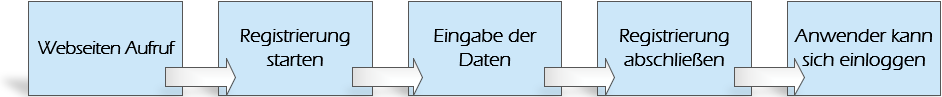
\includegraphics[width=1.0\textwidth]{06_Bilder/endtoend_test.png}
	\setlength{\abovecaptionskip}{0em}
	\caption{End-to-End (Beispiel Registrierungsprozess)}
	\label{img:endtoend_test}
\end{figure} 

\section{Selenium} \label{def:Selenium}
Wie bereits im Kapitel \ref{def:testpyramide} Testpyramide veranschaulicht, l�sst sich sehr gut erkennen, dass nur ein sehr geringer Teil aus Oberfl�chentests besteht. Um diese Tests zu automatisieren wurde im Jahre 2004 ein Framework namens Selenium entwickelt, mit dessen Hilfe es m�glich ist auf Webelemente zuzugreifen und mit ihnen zu interagieren. Selenium erm�glicht es, Tests auf Basis der Skriptsprache JavaScript, durchzuf�hren und unterst�tzt dabei mehrere \gls{browser}. Im Laufe der Entwicklung wurde Selenium immer weiter ausgebaut und unterst�tzt mittlerweile Programmiersprachen wie etwa Java, C\#, Ruby, Python und JavaScript. Mithilfe dieser Sprachen ist es m�glich das Framework zu verwenden und somit auf Webelemente zuzugreifen \autocite{selenium}. 

\subsection{Behavior Driven Development (\acs{BDD})} \label{def:BDD}
Oft f�llt es QA-Mitarbeitern und Abteilungen schwer einen guten Startpunkt in Bezug auf das Testen zu finden und genau zu definieren was alles getestet werden soll und was nicht. Ein Resultat aus dieser Erkenntnis ist, dass die Sprache in der Tests definiert werden eine wichtige Rolle spielen. Eine Technik der agilen Softwareentwicklung ist das sogenannte Behavior Driven Development (\acs{BDD}). Inspiriert durch \autocite{evans2004domain} nutzt \acs{BDD} nat�rliche Sprache, um Tests zu beschreiben. Mithilfe der nat�rliche Sprache wird gew�hrleistet, dass sowohl Stakeholder und Entwickler verstehen, um was es in diesem Test geht \autocite{soeken2012assisted}. 
\newline\newline
Da Selenium alleine nur eine Schnittstelle zwischen Webanwendungen und Tests darstellt, reicht Selenium nicht aus, um automatisierte Tests in nat�rlicher Sprache zu definieren. Aus diesem Grund gibt es die Beschreibungssprache \enquote{Gherkin}. Gherkin ist eine zeilenorientierte Sprache, die �hnlich wie Python Einz�ge zur Orientierung nutzt. Der \gls{parser} unterscheidet hierbei die Schl�sselw�rter \enquote{Feature}, \enquote{Scenario}, \enquote{Given}, \enquote{When}, \enquote{Then}, \enquote{And} und \enquote{But}. Je nach Framework kann die Sprache angepasst werden \autocite{gherkin}. Wenn beispielsweise Deutsch gew�hlt wird, werden die Schl�sselw�rter wie folgt angepasst:

\begin{itemize}
	\item Given 	-	Angenommen / Gegeben sei / Gegeben seien
	\item When	- 	Wenn
	\item Then	 -	 Dann
	\item And	 -	 Und
	\item But	 -	 Aber
\end{itemize}

Auf Basis von Gherkin gibt es Frameworks, die aufgrund der textuellen Spezifikation, mithilfe einer bestimmten Programmiersprache Tests automatisieren. Einige Beispiele sind:

\begin{itemize}
	\item Cucumber \autocite{cucumber}
	\item Lettuce \autocite{lettuce}
	\item Behave \autocite{behave}
\end{itemize}

\lstset{style=cypress, caption={Beispieltest Cucumber}, label={lst:cucumber}}
\begin{lstlisting}
# language: de
	
Funktionalit�t: Ein einfacher Test zur demonstration
	Dieser Test dient der Demonstration des Lesers, 
	damit dieser einen Eindruck davon erh�lt wie ein 
	Cucumber Test aussieht.
		
	Scenario: Demonstration
		Angenommen eine Tomate wiegt 100 Gramm
		Wenn ich diese Tomate halbiere
		Dann gibt es 2 St�cke mit je 50 Gramm
\end{lstlisting} 

Jede Zeile innerhalb eines Scenarios f�hrt eine Methode aus, die ein entsprechendes Ergebnis zur�ck gibt. Die ausf�hrbaren Methoden werden mithilfe einer Programmiersprache wie etwa Python, Ruby oder Java erstellt. Anzumerken ist hierbei, dass das verwendete \acs{BDD}-Framework die Programmiersprache unterst�tzen muss. Behave unterst�tzt beispielsweise nur Python \autocite{behave}. 
\newline\newline
Innerhalb dieser Methoden kann Selenium verwendet werden, um auf Webelemente zuzugreifen. So k�nnen beispielsweise mithilfe von Selenium, Werte aus Eingabefeldern oder Webelementen abgefragt werden. Diese Werte k�nnen entsprechend gegen gepr�ft werden. Entspricht ein Ergebnis nicht dem Erwarteten, wird das entsprechende Scenario mit einem Fehler abgebrochen \autocite{behave}.

\subsection{Pytest} \label{def:Pytest}
Doch nicht alle Frameworks nutzen Gherkin als Beschreibungssprache. Ein Beispiel hierf�r ist Pytest. Pytest l�sst sich nicht wie Gherkin lesen, sondern erh�lt �ber sogenannte \enquote{\glspl{fixture}} Objekte oder Werte die relevant f�r den jeweiligen Test sind. Anschlie�end werden Methoden Zeile f�r Zeile ausgef�hrt und daraus generierte Werte mithilfe von \enquote{\glspl{assertion}} gepr�ft \autocite{pytest}. Eine Assertion (englisch f�r Behauptung) ist die Aussage eines Zustandes innerhalb eines Programms. 

\newpage

\lstset{style=cypress, caption={fixture\_beispiel.py, enth�lt die Beispielfixture \enquote{port}}, label={lst:fixture}}
\begin{lstlisting}
import pytest

class WebKonfiguration:

	@pytest.fixture
	def port(self):
		return 80

\end{lstlisting} 

\lstset{style=cypress, caption={test\_beispiel.py, enth�lt den Test \enquote{test\_proof\_port}, assert True}, label={lst:pytest1}}
\begin{lstlisting}
from fixture_beispiel import WebKonfiguration

class Test(WebKonfiguration):

	def test_proof_port(self, port):
		assert port == 80

\end{lstlisting} 
In der Datei \enquote{fixture\_beispiel.py} (siehe Codebeispiel \ref{lst:fixture}) wird mithilfe des Befehls \enquote{class} eine Klasse gebildet, um eine Struktur zu schaffen (siehe Zeile 3). Anschlie�end wird eine \gls{fixture} mithilfe des \enquote{@pytest.fixture} Befehls erzeugt. Diese \gls{fixture} mit dem Namen \enquote{port}, generiert einen Wert, der zur�ckgegeben wird (Zeile 7).
\newline\newline
Die Datei \enquote{test\_beispiel.py} enth�lt die eigentlichen Tests (siehe Codebeispiel \ref{lst:pytest1}). �ber den Befehl \enquote{from fixture\_beispiel import WebKonfiguration} werden alle \glspl{fixture} der Klasse \enquote{WebKonfiguration} aus der Datei \enquote{fixture\_beispiel.py} importiert und somit nutzbar gemacht. Die soeben importierte Webkonfiguration wird an die Klasse \enquote{Test} �bergeben, damit sie von allen hierarchisch folgenden Tests genutzt werden kann.
\newline\newline
Der Test \enquote{test\_proof\_port} (siehe Codebeispiel \ref{lst:pytest1}) erh�lt �ber den �bergabeparameter \enquote{port} den R�ckgabewert der Fixture \enquote{port} (Wert 80, siehe Codebeispiel \ref{lst:fixture} Zeile 7). Innerhalb des Tests wird mithilfe des \enquote{assert}-Befehls �berpr�ft, ob der erwartete Wert dem aus der \gls{fixture} \enquote{port()} gleicht. 

\newpage

Ergibt dieser Vergleich True, wird w�hrend der Testausf�hrung folgende Ausgabe generiert:

\begin{figure}[H]
	\centering
	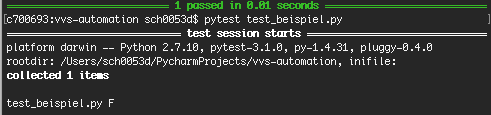
\includegraphics[width=1.0\textwidth]{06_Bilder/pytest_beispiel_true.png}
	\setlength{\abovecaptionskip}{0em}
	\caption{Pytest, Vergleich (Assert) ergibt True}
	\label{img:pytestexampletrue}
\end{figure} 

W�rde hingegen (siehe Codebeispiel \ref{lst:pytest2}) in Zeile sechs gegenteilig gepr�ft werden, ergibt sich folgendes:

\lstset{style=cypress, caption={test\_beispiel.py, enth�lt den Test \enquote{test\_proof\_port}, assert False}, label={lst:pytest2}}
\begin{lstlisting}
from fixture_beispiel import WebKonfiguration

class Test(WebKonfiguration):

	def test_proof_port(self, port):
		assert port != 80

\end{lstlisting} 

\begin{figure}[H]
	\centering
	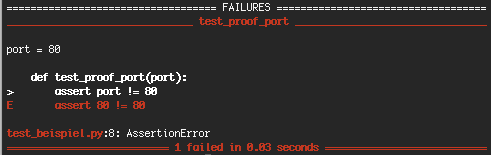
\includegraphics[width=1.0\textwidth]{06_Bilder/pytest_beispiel_false.png}
	\setlength{\abovecaptionskip}{0em}
	\caption{Pytest, Vergleich (Assert) ergibt False}
	\label{img:pytestexamplefalse}
\end{figure} 

Aus dem Kapitel \ref{def:BDD} geht hervor, dass alle erw�hnten Frameworks Selenium ben�tigen um auf Webelemente zuzugreifen (Siehe \autocite{cucumber}, \autocite{lettuce}, \autocite{behave}, \autocite{pytest}). QA-Mitarbeiter haben so zwar eine Auswahl verschiedener Programmiersprachen und Frameworks, sind allerdings bei der Erstellung der Oberfl�chentests f�r Webanwendungen auf Selenium angewiesen. 

\section{Cypress}
Cypress, auch Cypress.io genannt, versucht ein Gesamtpaket zur Erstellung von Oberfl�chentests f�r Webanwendungen anzubieten. Anders als alle Frameworks die in Kapitel \ref{def:BDD} beschrieben wurden, ist Cypress nicht auf Selenium angewiesen und verspricht vor allem das Erstellen, Schreiben, Ausf�hren und Debuggen von Tests zu vereinfachen. Da es ebenfalls ein Funktions- und Akzeptanztesttool f�r Webanwendungen ist, wird es h�ufig mit Selenium verglichen \autocite{cypress}. 
\newline\newline
Standardm��ig bringt Cypress den sogenannten \enquote{Cypress Test Runner} mit. Dieser listet alle verf�gbaren Tests auf, zeigt Testdurchl�ufe an und ist in der Lage ein Cypress Projekt �ber die Einstellungen individuell anzupassen. Zus�tzlich ist es m�glich die aufgelisteten Tests in einem ausgew�hlten Browser laufen zu lassen. W�hrend der Ausf�hrung, wird im Browser in einer Spalte der Ablauf in Echtzeit �bersichtlich dargestellt \autocite{cypress}. 
\\

\begin{figure}[H]
	\centering
	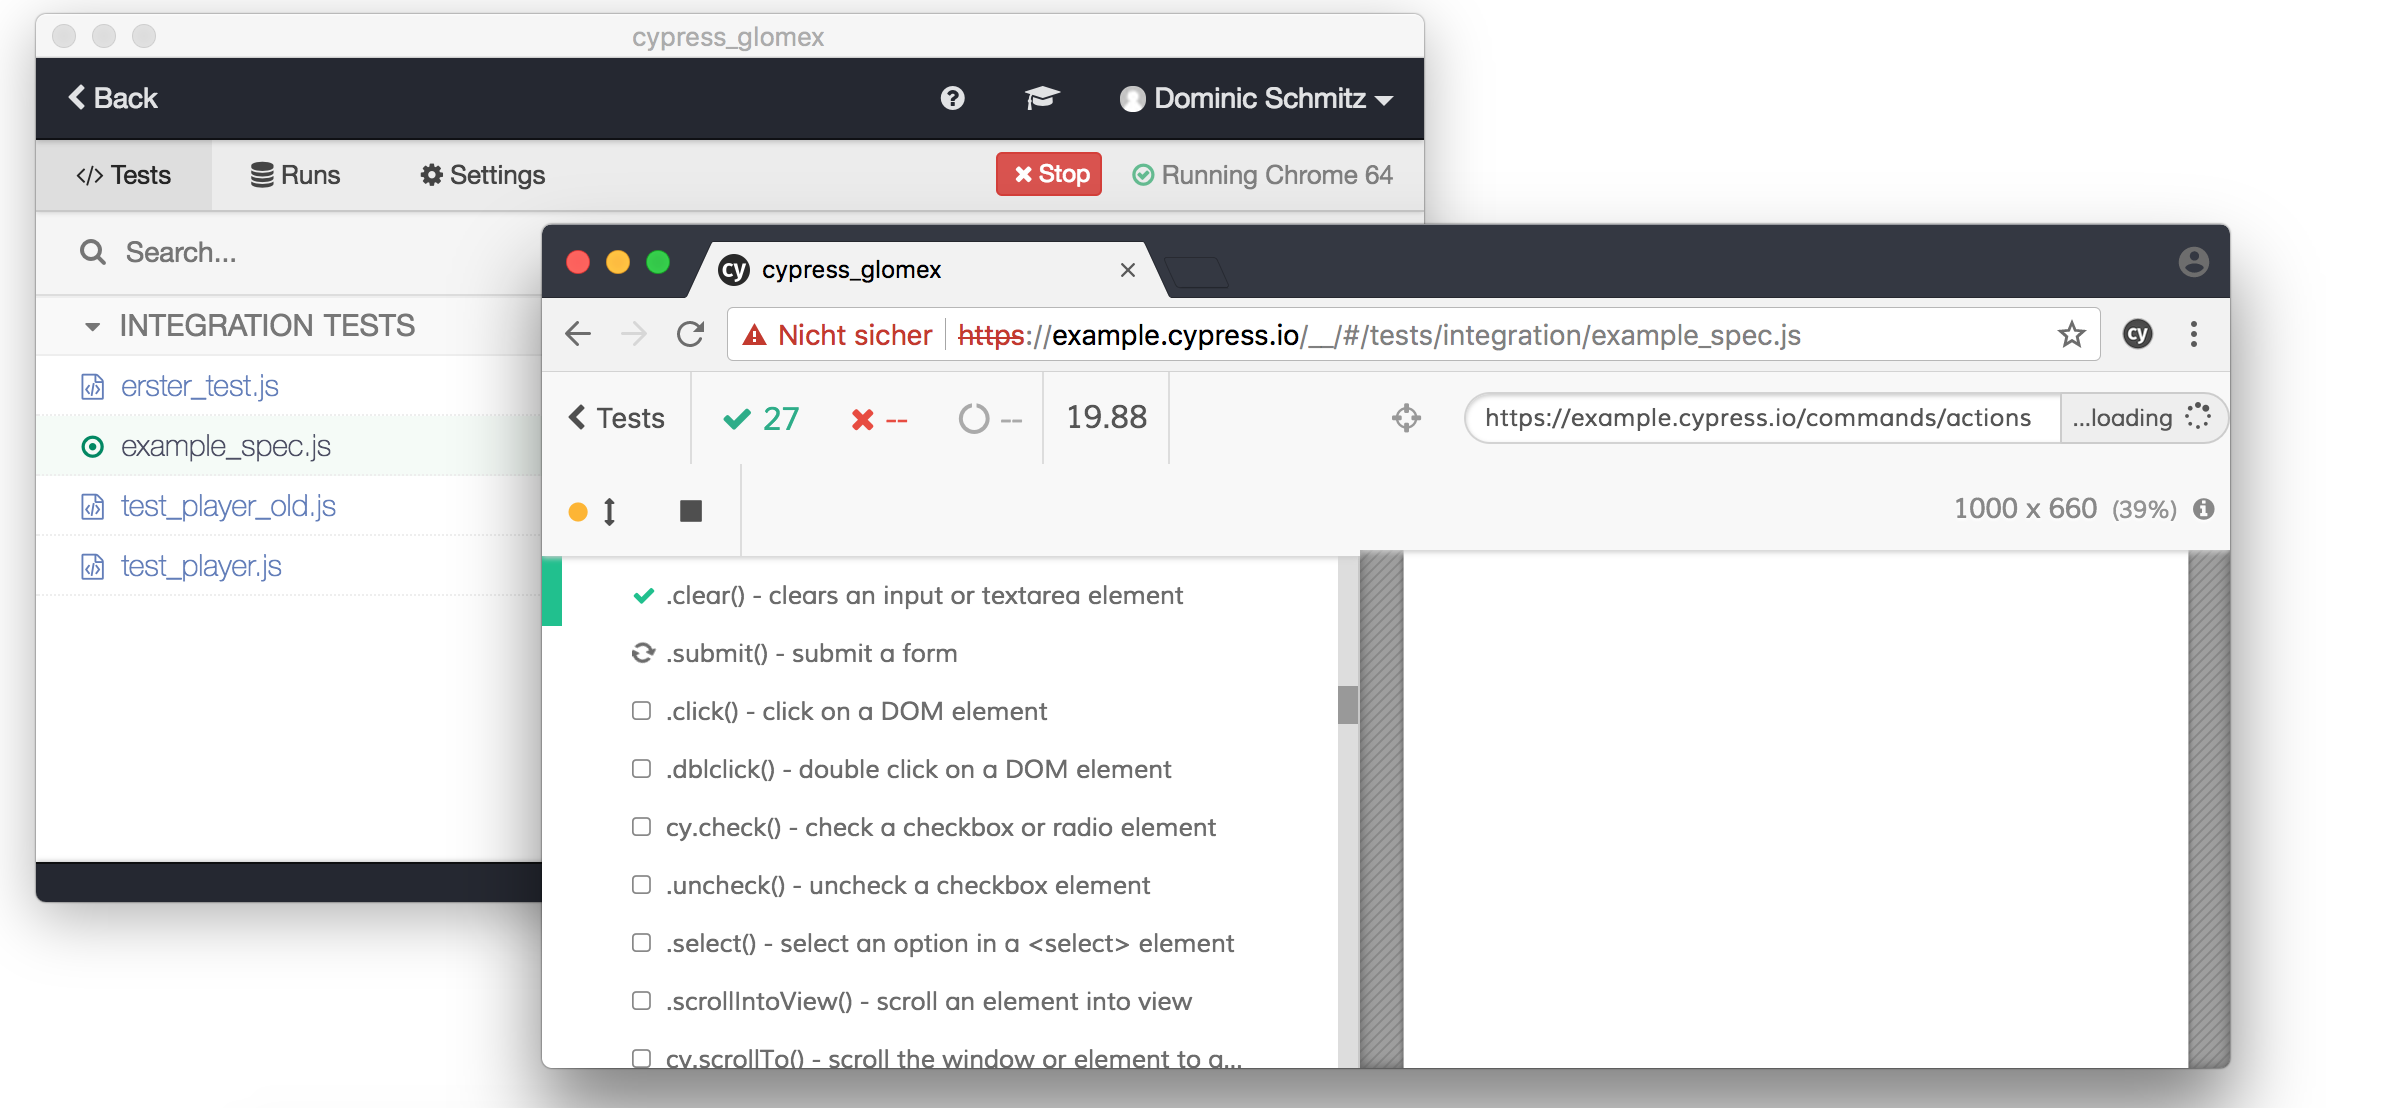
\includegraphics[width=1.0\textwidth]{06_Bilder/cypress_running_test.png}
	\setlength{\abovecaptionskip}{0em}
	\caption{Cypress Test Runner w�hrend einer Testausf�hrung}
	\label{img:cypress_test_runner}
\end{figure} 


% !TEX root = Installation.tex

\chapter{Installation / Konfiguration} \label{def:installation}
Damit beide Frameworks miteinander verglichen werden k�nnen, muss zun�chst Cypress installiert werden. Die bestehende Selenium-Pytest Infrastruktur existiert bereits im Unternehmen und muss nur mithilfe des Versionsverwaltungstools Git, heruntergeladen werden. 
\newline\newline
In diesem Kapitel wird beschrieben, wie die Installation und Konfiguration von Cypress stattfindet. Zus�tzlich werden die Voraussetzungen zur Installation von Cypress erl�utert und welches System zur Testautomatisierung im Rahmen dieser Arbeit verwendet wird.

\section{Umgebung}
Das Unternehmen glomex ben�tigt ein System, dass alle Anforderungen unterst�tzt. Die Umgebung muss von Cypress.io sowie von Selenium unterst�tzt werden. 
\newline\newline
Cypress wird derzeit (Stand 13.02.2018) auf folgenden Plattformen supportet \autocite{cypress}:
\begin{itemize}
	\item Mac OS 10.9+ (Mavericks+), only 64bit binaries are provided for macOS.
	\item Linux Ubuntu 12.04+, Fedora 21, Debian 8.
	\item Windows 7+, only 32bit binaries are provided for Windows.
\end{itemize}

Selenium setzt nur einen installierten Browser und eine der folgenden Programmiersprachen voraus \autocite{selenium}:
\begin{itemize}
	\item Java
	\item C\# 
	\item Ruby
	\item Python
	\item Javascript (Node)
\end{itemize}

Da unternehmensweit bei der glomex Mac OS genutzt wird und beide Frameworks, sowohl Cypress als auch Selenium unterst�tzt werden, wurde entschieden Mac OS zu verwenden. 

\section{Cypress Test Runner} \label{def:cypress_test_runner}
\subsection{Installation unter Mac OS}

\begin{figure}[H]
	\centering
	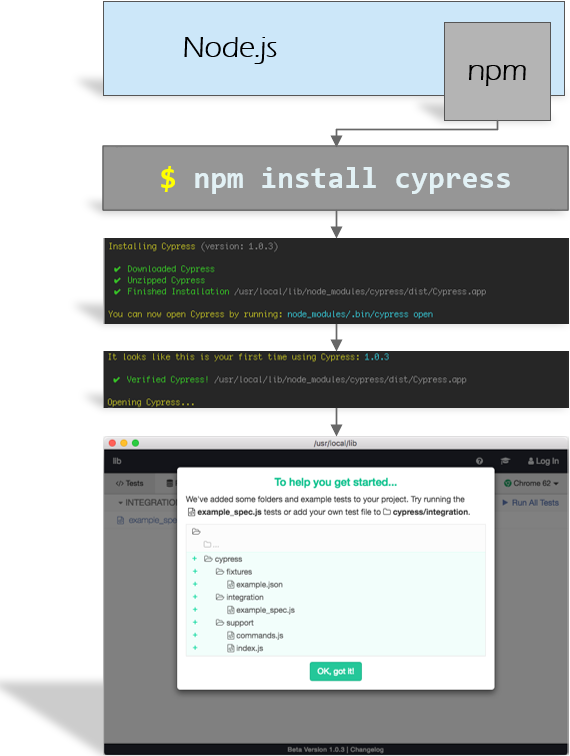
\includegraphics[width=0.98\textwidth]{06_Bilder/cypress_installationsprozess.png}
	\setlength{\abovecaptionskip}{1em}
	\caption{Cypress Installationsprozess (Mac OS)}
	\label{img:cypress_install_grafik}
\end{figure}

Bei der Verwendung von Mac OS muss erst das Programm \enquote{Node.js} installiert werden, da dieses den \gls{packagemanager} Npm enth�lt (siehe Abbildung \ref{img:cypress_install_grafik}). Npm ist ein \gls{packagemanager} f�r JavaScript und enth�lt tausende frei zum Download verf�gbare Pakete \autocite{npm}. F�r das Betriebssystem Mac OS wird empfohlen, Cypress mithilfe von Npm zu installieren, da Npm in der Lage ist, Cypress zu aktualisieren und zu installieren \autocite{cypress}.  
\newline\newline
Nach der Installation steht der Befehl \enquote{npm} in einer eingabebasierenden Benutzerschnittstelle der sogenannten \gls{bash} zur Verf�gung. Mithilfe des Befehls \enquote{npm install cypress} kann nun die Installation des Cypress Test Runners gestartet werden (siehe Abbildung \ref{img:cypress_install_grafik}). 

\subsection{Konfiguration} \label{def:konfiguration}
Nach Abschluss der Installation ist der sogenannte \enquote{Cypress Test Runner} installiert. Dieser enth�lt alle wichtigen Tools und Einstellungen um Tests zu starten und Ergebnisse auszuwerten.
\newline\newline
Es gibt zwei Wege den Cypress Test Runner zu starten:

\begin{itemize}
	\item \textbf{Mithilfe des \gls{bash}befehls \enquote{node\_modules/.bin/cypress open} (siehe Abbildung \ref{img:cypress_install_grafik})}\\
	Dabei ist zu beachten, dass der Befehl nur funktioniert, wenn der Anwender sich im Cypress Projektverzeichnis befindet. Zus�tzlich ist der Anwender mit dieser Methode nicht in der Lage das Projektverzeichnis auszuw�hlen.
	\item \textbf{Direkt �ber Programme}\\
	Bei dieser Methode kann der Anwender selber ein vorhandenes Projektverzeichnis ausw�hlen oder ein neues erstellen.

\end{itemize}

\subsection{Update} \label{def:cypress_update}
Cypress �berpr�ft vor jedem Start ob eine neue Version verf�gbar ist. Sobald eine neue Version zur Verf�gung steht, erscheint ein Update-Button im unteren Bereich des Cypress Test Runners. �ber diesen Button wird einem explizit angezeigt, welche Schritte der Anwender zu gehen hat, damit Cypress aktualisiert wird. 

\begin{figure}[H]
	\centering
	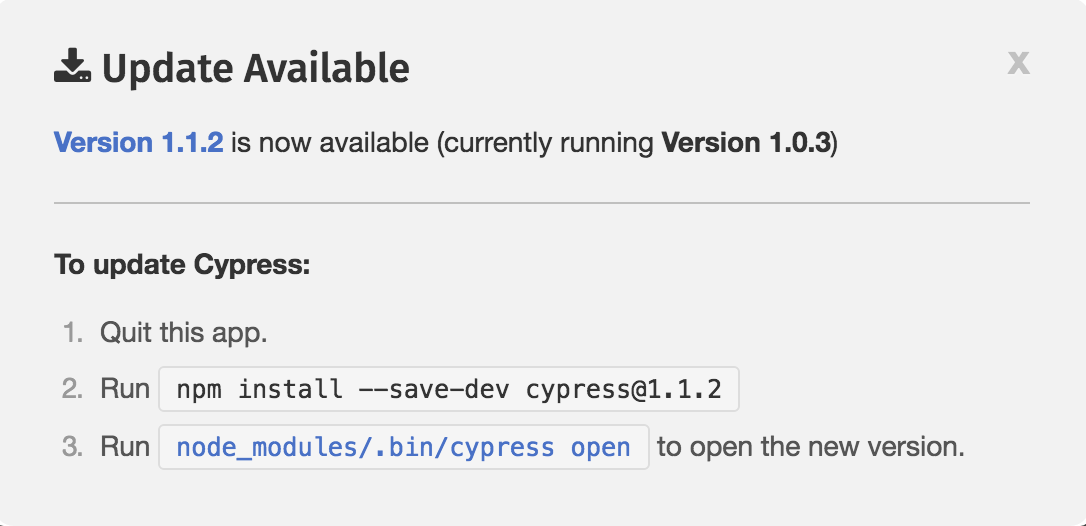
\includegraphics[width=1.0\textwidth]{06_Bilder/cypress_update.png}
	\setlength{\abovecaptionskip}{0em}
	\caption{Cypress Update}
	\label{img:cypress_update}
\end{figure}

Nachdem das Update durchgef�hrt wurde, kann die neue Version des Cypress Test Runners, wie in Kapitel \ref{def:konfiguration} beschrieben, gestartet werden.

\section{Visual Studio Code} \label{def:visual_studio}
Sobald der Cypress Test Runner installiert wurde, wird noch zus�tzlich ein Editor zum Erstellen und Editieren der Tests in Form von JavaScript (.js) Dateien ben�tigt. Im Rahmen dieser Arbeit wurde entschieden \enquote{Visual Studio Code} zu verwenden, da dieser Editor alle g�ngigen Plattformen unterst�tzt und ein \gls{syntax} f�r JavaScript beinhaltet. Im Vergleich zur Installation des Cypress Test Runners, muss nur eine Installationsdatei heruntergeladen und installiert werden \autocite{visualstudio}. 
% !TEX root = Einfuehrung.tex

\chapter{Cypress Einf�hrung}
Um mit Cypress effektiv Tests zu erstellen, muss erst verstanden werden, wie ein Cypress Projekt grunds�tzlich aufgebaut ist. Die in diesem Kapitel beschriebene Struktur wird von Cypress empfohlen. Es ist m�glich diese Struktur anzupassen und zu ver�ndern. Im Rahmen dieser Arbeit wird darauf allerdings verzichtet. Zus�tzlich werden in diesem Abschnitt die wichtigsten Kommandos erl�utert.

\section{Projektstruktur} \label{def:cypress_projektstruktur}
Die von Cypress empfohlene Struktur wird bereits beim ersten Anlegen eines Projektes erstellt. �nderungen k�nnen mithilfe des Cypress Test Runners �ber die Einstellungen konfiguriert werden. 
\newline\newline
Beim ersten Start des Cypress Test Runners kann ein Projektordner ausgew�hlt werden. Wird ein Ordner gew�hlt, wird gepr�ft, ob bereits eine cypress.json Datei vorhanden ist. Diese Datei enth�lt die Project ID mithilfe dieser das Projekt einer Organisation zugeordnet werden kann (siehe \ref{def:cypress_dashboard}). Ist diese Datei nicht enthalten, erstellt Cypress ein neues Projekt mit der folgenden Struktur:

\begin{figure}[H]
	\centering
	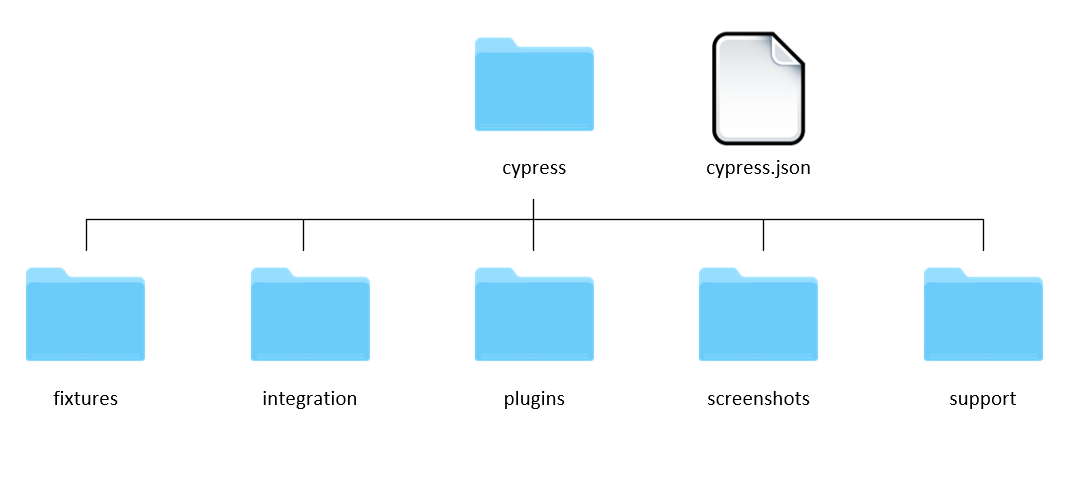
\includegraphics[width=1.0\textwidth]{06_Bilder/cypress_ordner_hierarchie.png}
	\setlength{\abovecaptionskip}{-1em}
	\caption{Cypress Projektstruktur}
	\label{img:cypress_folder}
\end{figure}

Neben einer cypress.json Datei wird der Ordner cypress erstellt, der die Ordner \enquote{fixtures}, \enquote{integration}, \enquote{plugins}, \enquote{screenshots} und \enquote{support} enth�lt (siehe Abbildung \ref{img:cypress_folder}). Standardm��ig enth�lt jeder Ordner Beispieldateien.
\newpage

\begin{itemize}
	\item \textbf{fixtures}\\
	Der Ordner fixtures enth�lt json Dateien. Das Format json ist ein schlankes Datenaustauschformat, dass f�r Menschen einfach zu lesen und zu schreiben ist \autocite{json}. Cypress verwendet diese Dateien dazu Werte zu speichern, die wiederholt f�r Tests ben�tigt werden. Jeder Test kann eine oder mehrere fixtures implementieren, um gespeicherte Werte wiederholt abzurufen.
	
	\lstset{style=cypress, caption={Fixture json Beispiel (Quelle: \autocite{cypress})}, label={lst:fixture_beispiel}}
	\begin{lstlisting}
	{
		"name": "Using fixtures to represent data",
		"email": "hello@cypress.io"
	}
	\end{lstlisting} 
			
	\item \textbf{integration}\\
	Eine der wichtigsten Funktionen �bernimmt der Ordner \enquote{integration}. In diesem Ordner werden alle Tests in Form von JavaScript Dateien (.js) gespeichert. Cypress basiert auf der Skriptsprache JavaScript und verwendet diese zur Erstellung von Tests \autocite{cypress}. 
	
	\item \textbf{plugins}\\
	Plugins erlauben dem Benutzer das grundlegende Verhalten von Cypress zu ver�ndern oder zu erweitern. Sie sind eine Nahtstelle, um eigenen benutzerdefinierten Code zu schreiben und diesen w�hrend bestimmter Phasen eines Tests auszuf�hren \autocite{cypress}. 
	
	\item \textbf{screenshots}\\
	Um zu gew�hrleisten, dass bestimmte Zust�nde erreicht wurden, k�nnen zur Sicherheit Screenshots w�hrend des Testablaufs erstellt werden. Ein Screenshot ist eine Momentaufnahme, die in der Regel als Bild gespeichert wird. Dieses Bild wird in dem Ordner \enquote{screenshots} gespeichert und kann entsprechend nach dem Testablauf aufgerufen werden \autocite{cypress}.   
	
	\item \textbf{support}\\
	Innerhalb des Ordners \enquote{support}, befindet sich die Datei index.js. Diese Datei bestimmt, welcher Code automatisch vor jeder Testausf�hrung geladen wird. So k�nnen beispielsweise bestimmte Kommandos erstellt, in einer Datei gespeichert und mithilfe der index.js vor jeder Testausf�hrung automatisch geladen werden. So kann ein selbst definiertes Kommando f�r jeden Test bereitgestellt werden \autocite{cypress}. 
	
\end{itemize}

Im Rahmen dieser Arbeit ist seitens der glomex gew�nscht, die in Abbildung \ref{img:cypress_folder} verwendete Struktur beizubehalten. Alle Cypress Tests, die in dieser Arbeit erstellt und ausgef�hrt werden, verwenden die beschriebene Struktur. 


\section{Blockstrukturen}
Um einen Test zu erstellen, wird eine neue JavaScript Datei (.js) mithilfe Visual Studio Code (siehe Kapitel \ref{def:visual_studio}) innerhalb des \enquote{integration} Ordners (siehe Abbildung \ref{img:cypress_folder}) erstellt. Jeder Cypress Test besitzt eine definierte Struktur. Diese enth�lt grundlegend einen \enquote{describe Block}, der beschreibt, um was f�r einen Test es sich handelt. Innerhalb des \enquote{describe Blocks} k�nnen nun folgende Konstrukte verwendet werden:

\begin{itemize}
	\item \textbf{it}\\
	Ein sogenannter \enquote{it Block} repr�sentiert einen Test. In ihm befinden sich alle Kommandos die zur Abarbeitung des Tests ben�tigt werden \autocite{cypress}. 
	
	\lstset{style=cypress, caption={it Block}, label={lst:it_block}}
	\begin{lstlisting}
	describe('describe Block', function() {
		it('Demonstriert einen it Block', function() {
			// Hier Kommandos
		})
	})
	\end{lstlisting} 
	
	\item \textbf{context}\\
	\enquote{context Bl�cke} enthalten Tests und dienen der �bersichtlichkeit. Aus diesem Grund k�nnen \enquote{context Bl�cke} \enquote{it Bl�cke} und weitere Konstrukte enthalten. Die Aufteilung in \enquote{context Bl�cke} hat den Vorteil, dass mithilfe eines \enquote{describe Blocks} ein Gebiet definiert werden kann, in dem mehrere \enquote{Context Bl�cke} abgearbeitet werden \autocite{cypress}. 
	\newline\newline 
	Ein Beispiel w�re ein Test eines glomex Video Players. So kann als \enquote{describe Block} \enquote{Player Test} definiert werden. Innerhalb dieses Blocks k�nnen nun verschiedene Videoplayer mithilfe der \enquote{context Bl�cke} getestet werden. 
	
	\newpage
	
	\lstset{style=cypress, caption={context Block}, label={lst:context_block}}
	\begin{lstlisting}
	describe('Player Test', function() {
	
		context('Flash Player', function() {
			it('Pause Test', function() {
				// Kommandos um Pause im Flash Player zu testen
			})
		})
		
		context('HTML Player', function() {
			it('Pause Test', function() {
				// Kommandos um Pause im HTML Player zu testen
			})
		})
		
	})
	\end{lstlisting} 
	
	\begin{figure}[H]
		\centering
		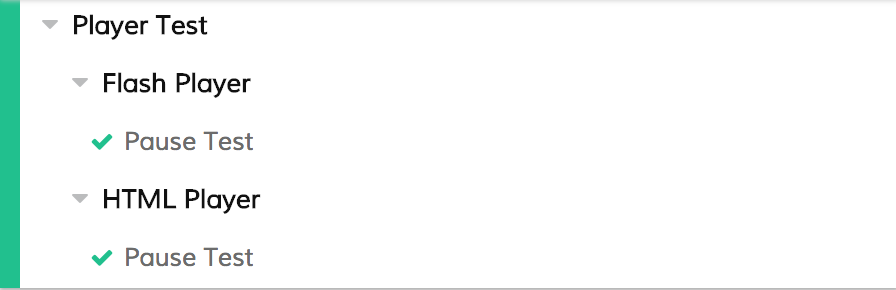
\includegraphics[width=1.0\textwidth]{06_Bilder/cypress_context.png}
		\setlength{\abovecaptionskip}{0em}
		\caption{Cypress Test Struktur}
		\label{img:cypress_context}
	\end{figure}

	\item \textbf{before und beforeEach}\\
	Um Code vor einem oder mehreren Tests auszuf�hren, werden sogenannte \enquote{before} oder \enquote{beforeEach} Bl�cke verwendet. Der Unterschied zwischen diesen beiden Bl�cken ist, dass der \enquote{before Block} nur einmalig vor dem n�chst folgenden \enquote{it Block} ausgef�hrt wird. Hingegen wird der \enquote{beforeEach Block} vor jedem \enquote{it Block} der hierarchisch folgt erneut abgearbeitet. Beide Bl�cke k�nnen in jeder Hierarchieebene verwendet werden.
	
	\newpage
	
	\lstset{style=cypress, caption={before und beforeEach BBlock}, label={lst:before_block}}
	\begin{lstlisting}
	describe('Player Test', function() {
	
		before(function(){
			/*
			Wird nur vor "Flash Player - Pause Test" 
			ausgef�hrt, da es sich um den n�chst
			hierarischen Test handelt.
			*/
		})
	
		beforeEach(function(){
			/* 
			Wird vor jedem hirarisch folgenden Test
			ausgef�hrt. In diesem Fall vor:
	
			- Flash Player - Pause Test
			- HTML Player - Pause Test 
			*/
		})
	
		context('Flash Player', function() {
			it('Pause Test', function() {
				// Kommandos um Pause im Flash Player zu testen
			})
		})
	
		context('HTML Player', function() {
			it('Pause Test', function() {
				// Kommandos um Pause im HTML Player zu testen
			})
		}) 
	})
	\end{lstlisting} 
\end{itemize}

\section{Wichtige Kommandos}
Tests arbeiten eine Folge von Kommandos sequentiell ab. Cypress stellt eine reihe dieser Kommandos zur Verf�gung, von denen jedes eine bestimmte Funktionalit�t �bernimmt. In diesem Abschnitt werden nur Kommandos mit Relevanz f�r diese Arbeit erl�utert. Unter \autocite{cypress} kann eine vollst�ndige Kommandoliste eingesehen werden.

\begin{itemize}
	\item \textbf{cy.visit(URL)}\\
	Mithilfe des \enquote{visit} Befehls wird eine Webseite aufgerufen. \vspace{0.8em}\\
	\textbf{Beispiel:}
	\lstset{style=cypress,caption={Ruft die Webseite \enquote{www.google.de} auf}, label={lst:visit}, aboveskip=0.4em, belowskip=1em, abovecaptionskip=0.4em}
	\begin{lstlisting}
		cy.visit(www.google.de)
	\end{lstlisting} 
	
	\item \textbf{cy.wait(Zeit)}\\
	Der Befehl \enquote{wait} pausiert einen Test f�r eine bestimmte Zeit. Die Zeit wird in Millisekunden angegeben. \vspace{0.8em}\\
	\textbf{Beispiel:}
	\lstset{style=cypress,caption={Wartet eine Sekunde bis der Test fortgef�hrt wird}, label={lst:wait}, aboveskip=0.4em, belowskip=1em, abovecaptionskip=0.4em}
	\begin{lstlisting}
		cy.wait(1000)
	\end{lstlisting} 
	
	\item \textbf{cy.get(Locator)}\\
	Um auf ein Webelement zuzugreifen gibt es den \enquote{get} Befehl. Dieser gibt ein oder mehrere Webelemente einer Webseite zur�ck. \vspace{0.8em}\\
	\textbf{Beispiel:} 
	\lstset{style=cypress,caption={Gibt einen Playback Button zur�ck}, label={lst:get}, aboveskip=0.4em, belowskip=1em, abovecaptionskip=0.4em}
	\begin{lstlisting}
		cy.get(button[data-qa=playbackButton])
	\end{lstlisting}
	
	\newpage
	
	\item \textbf{.click()}\\
	Es gibt Befehle, die nur mithilfe Weiterer funktionieren. Der Befehl click() klickt ein Webelement. Da das Webelement erst gefunden werden muss, um geklickt werden zu k�nnen, wird der Befehl get (siehe Codebeispiel \ref{lst:get}) vorausgesetzt. \vspace{0.8em}\\
	\textbf{Beispiel:} 
	\lstset{style=cypress,caption={Klickt den Playback Button}, label={lst:click}, aboveskip=0.4em, belowskip=1em, abovecaptionskip=0.4em}
	\begin{lstlisting}
	cy.get(button[data-qa=playbackButton]).click()
	\end{lstlisting}
	
	\item \textbf{.should(Bedingung)}\\
	Zus�tzlich zum \enquote{get} Befehl k�nnen weitere Bedingungen mithilfe des \enquote{should} Befehls angegeben werden, um ein Webelement genau zu spezifizieren. Trifft diese Bedingung nicht innerhalb einer bestimmten Zeit zu, wird der Test mit einem Fehler beendet (siehe \gls{assertion}). \vspace{0.8em}\\
	\textbf{Beispiel:} 
	\lstset{style=cypress,caption={Sucht nach einem \enquote{sichtbaren} Playback Button}, label={lst:should}, aboveskip=0.4em, belowskip=1em, abovecaptionskip=0.4em}
	\begin{lstlisting}
		cy.get(button[data-qa=playbackButton])
			.should('be.visible')
	\end{lstlisting}
	
	\item \textbf{.find(Locator)}\\
	Das Kommando \enquote{find}, findet ein Webelement innerhalb eines Webelements. \vspace{0.8em}\\
	\textbf{Beispiel:} 
	\lstset{style=cypress,caption={Finde \enquote{footer} innerhalb \enquote{article}}, label={lst:find}, aboveskip=0.4em, belowskip=1em, abovecaptionskip=0.4em}
	\begin{lstlisting}
		cy.get('.article').find('footer')
	\end{lstlisting}
	
	\item \textbf{cy.screenshot(Name)}\\
	Um einen Screenshot zu erstellen, muss der Befehl \enquote{screenshot} ausgef�hrt werden. Als Parameter muss ein Name �bergeben werden, unter dem dieser gespeichert wird. Der erstellte Screenshot wird in dem Ordner \enquote{screenshots} (siehe Abbildung \ref{img:cypress_folder}) als Bilddatei abgespeichert. \vspace{0.8em}\\
	\textbf{Beispiel:} 
	\lstset{style=cypress,caption={Erstellt ein Bild mit dem Namen \enquote{Bildname} im Ordner \enquote{screenshots}}, label={lst:screenshot}, aboveskip=0.4em, belowskip=1em, abovecaptionskip=0.4em}
	\begin{lstlisting}
		cy.screenshot('Bildname')
	\end{lstlisting}
	
	\newpage
		
	\item \textbf{cy.log(Meldung)}\\
	Jeder Test gibt w�hrend der Ausf�hrung einen Eventlog aus. Mithilfe des \enquote{log} Befehls kann eine Meldung erzeugt und zur Laufzeit im Eventlog ausgegeben werden. \vspace{0.8em}\\
	\textbf{Beispiel:} 
	\lstset{style=cypress,caption={Schreibt \enquote{Dies ist eine Meldung} in den Log}, label={lst:log}, aboveskip=0.4em, belowskip=1em, abovecaptionskip=0.4em}
	\begin{lstlisting}
	cy.log(Dies ist eine Meldung)
	\end{lstlisting}
	
	\item \textbf{cy.reload()}\\
	Der Befehl \enquote{reload} l�dt die Webseite neu, auf der sich der Test Momentan befindet. \vspace{0.8em}\\
	\textbf{Beispiel:} 
	\lstset{style=cypress,caption={L�dt die Seite neu}, label={lst:reload}, aboveskip=0.4em, belowskip=1em, abovecaptionskip=0.4em}
	\begin{lstlisting}
		cy.reload()
	\end{lstlisting}
	
	\item \textbf{cy.scrollTo(Position)}\\
	Mithilfe des \enquote{scrollTo} Kommandos scrollt der Test an eine angegebene Position. Es k�nnen xy Koordinaten als Position verwendet werden oder direkte Befehle wie etwa top, right, left oder bottom. \vspace{0.8em}\\
	\textbf{Beispiel:} 
	\lstset{style=cypress,caption={Scrollt bis an den Anfang (top) der Webseite}, label={lst:reload}, aboveskip=0.4em, belowskip=1em, abovecaptionskip=0.4em}
	\begin{lstlisting}
		cy.scrollTo('top')
	\end{lstlisting}
	
	\item \textbf{cy.wrap(subject)}\\
	Der Befehl \enquote{wrap}, zu Deutsch \enquote{wickeln} oder auch \enquote{verpacken} legt ein zu nutzendes Objekt fest. Mithilfe von invoke kann mit dem Objekt interagiert werden.\vspace{0.8em}\\
	\textbf{Beispiel:} 
	\lstset{style=cypress,caption={Holt den Namen \enquote{Jane Lane}}, label={lst:wrap}, aboveskip=0.4em, belowskip=1em, abovecaptionskip=0.4em}
	\begin{lstlisting}
		cy.wrap({ name: "Jane Lane" })
		  .invoke('name').should('eq', 'Jane Lane') // true
	\end{lstlisting}
	
\end{itemize}
% !TEX root = Automatisierung.tex

\chapter{Automatisierung der Ausf�hrung}

\section{Testimplementierung in Travis}
In diesem Kapitel wird erl�utert, was Travis ist und inwiefern damit Cypress Tests automatisiert werden k�nnen. Zus�tzlich wird n�her auf das Cypress Dashboard eingegangen.

\subsection{Travis}
Mit Travis ist es m�glich Software Tests automatisiert auszuf�hren. Travis kann mit einem �ffentlichen (kostenfrei) oder einem privaten (Kostenpflichtig) Github \gls{repository} verkn�pft werden. Die Website hat daf�r zwei unterschiedliche Domains bereitgestellt. travis-ci.org f�r �ffentliche Projekte und travis-ci.com f�r private Projekte. Jedes Mal wenn eine �nderung des Codes auf dem verkn�pften Github-\gls{repository} stattfindet, l�sst sich mithilfe von Konfigurationsdateien bestimmen, welche Anweisungen erfolgen. Diese Anweisungen m�ssen nicht zwingend das Ausf�hren von Tests enthalten, es k�nnen auch Anweisungen zum Versenden von Nachrichten oder Erstellen von Berichten sein \autocite{travis}.

\subsection{Git / Github}

\begin{itemize}
	\item \textbf{Git}\\
	Git ist ein System zur verteilten Versionsverwaltung mehrerer Dateien. Es wurde unter den Aspekten Geschwindigkeit, einfaches Design, guter Unterst�tzung von nicht-linearer Entwicklung, vollst�ndiger Verteilung und der F�higkeit gro�e Projekte effektiv zu verwalten entwickelt. Das Prinzip besteht darin, den Zustand einer oder mehrerer Dateien zu sichern und diese sogenannten \glspl{snapshot}, unter einer Referenz abzuspeichern. Bei diesem Vorgang werden unver�nderte Dateien nicht erfasst, es wird lediglich eine Verkn�pfung zu der Datei erstellt. Durch diese Vorgehensweise wird die Effizienz und Geschwindigkeit besonders bei gro�en Projekten enorm gesteigert. Ein weiterer gro�er Vorteil ist die M�glichkeit einen \gls{branch} zu erstellen. Ein \gls{branch} in Git ist ein simpler Zeiger, der auf einen Codestand verweist. Er erm�glicht es, an mehreren Codest�nden zur selben Zeit zu entwickeln und diese sp�ter zusammenzuf�hren \autocite{gitbook}.
	
	\item \textbf{Github}\\
	Github ist eine im Jahre 2007 in San Francisco gegr�ndete Website, mit der es m�glich ist Entwicklungsprojekte anzulegen und zu verwalten. In sogenannten \glspl{repository} werden Daten und Codest�nde verschiedener Projekte gespeichert und k�nnen mithilfe der Versionsverwaltung Git abgerufen und ver�ndert werden \autocite{github}.
	
\end{itemize}

\subsection{Testimplementierung}
Um Travis nutzen zu k�nnen, m�ssen im ersten Schritt folgende Voraussetzungen erf�llt werden \autocite{travisStart}:

\begin{itemize}
	
	\item GitHub login
	\item Zu automatisierendes Projekt, bereitgestellt auf einem GitHub-\gls{repository}
	\item Lauff�higer Code im Projekt
	\item Lauff�higer Stand oder Testscript
	
\end{itemize}

Nachdem alle Voraussetzungen erf�llt sind, kann nun der Travis Login stattfinden. Hierbei ist zu beachten, dass die Zugriffsvereinbarungen akzeptiert werden, da Travis sonst keinen Zugriff auf das zu automatisierende Projekt erh�lt. Anschlie�end kann direkt �ber die eigenen Profileinstellungen das GitHub-\gls{repository} mit dem lauff�higen Code ausgew�hlt werden. �ber diese Einstellung kann auch konfiguriert werden, wann Tests automatisiert ausgef�hrt werden sollen. Im Rahmen dieser Arbeit wurde eine Testausf�hrung, einmal am Tag und immer wenn der Master Branch des Github-\glspl{repository} ver�ndert wurde, eingestellt.
\\\\
Im n�chsten Schritt muss eine Datei mit dem Namen \enquote{.travis.yml} im Hauptverzeichnis des GitHub-\glspl{repository} erstellt werden. Mithilfe dieser Datei erh�lt Travis Informationen dar�ber, was w�hrend einer Testausf�hrung geschehen soll.

	\lstset{style=travis, caption={Travis Konfigurationsdatei (.travis.yml)}, label={lst:travis.yml}}
\begin{lstlisting}
language: node_js

node_js:
	- 6

cache:
	directories:
		- ~/.npm
		- node_modules

install:
	- npm install cypress --save-dev

before_script:
	- npm start -- --silent &
		
script:										  
	- cypress run --record --key 12345678-90ab-cdef-1234-567890abcdef --spec cypress/integration/test_player.js
\end{lstlisting} 

Die Hauptparameter des Codebeispiels \ref{lst:travis.yml} wurden der Webseite \autocite{cypressTravisYml} entnommen. Wichtig hierbei ist vor allem die Angabe des Tests in Zeile 18. Dabei �bernehmen die folgenden Parameter, bestimmte Aufgaben.

\begin{itemize}
	
	\item \textbf{--record}\\
	Mithilfe von --record, ist der Test in der Lage ein Video oder Screenshots des Testablaufs zu erstellen. Diese k�nnen �ber das Cypress Dashboard angesehen oder heruntergeladen werden (siehe Kapitel \ref{def:cypress_dashboard}).
	
	\item \textbf{--key}\\
	Um Videos und Screenshots einem Cypress Account zuzuordnen, gibt es den --key Parameter. Ein Key kann �ber das Cypress Dashboard generiert und muss bei der Testausf�hrung mit angegeben werden. 
	
	\item \textbf{--spec}\\
	Durch die Angabe von --spec, wird genau spezifiziert, welcher Test ausgef�hrt werden soll. Wird der Parameter nicht angegeben, werden alle Tests die sich in dem Ordner integration befinden, chronologisch abgearbeitet. 
	
\end{itemize}

Alle bisher ausgef�hrten Tests k�nnen auch �ber die Weboberfl�che h�ndisch neu gestartet werden. Zus�tzlich gibt es einen Log, der den genauen Ablauf eines jeden Tests genau dokumentiert (siehe Abbildung \ref{img:travis_log}). 

\begin{figure}[H]
	\centering
	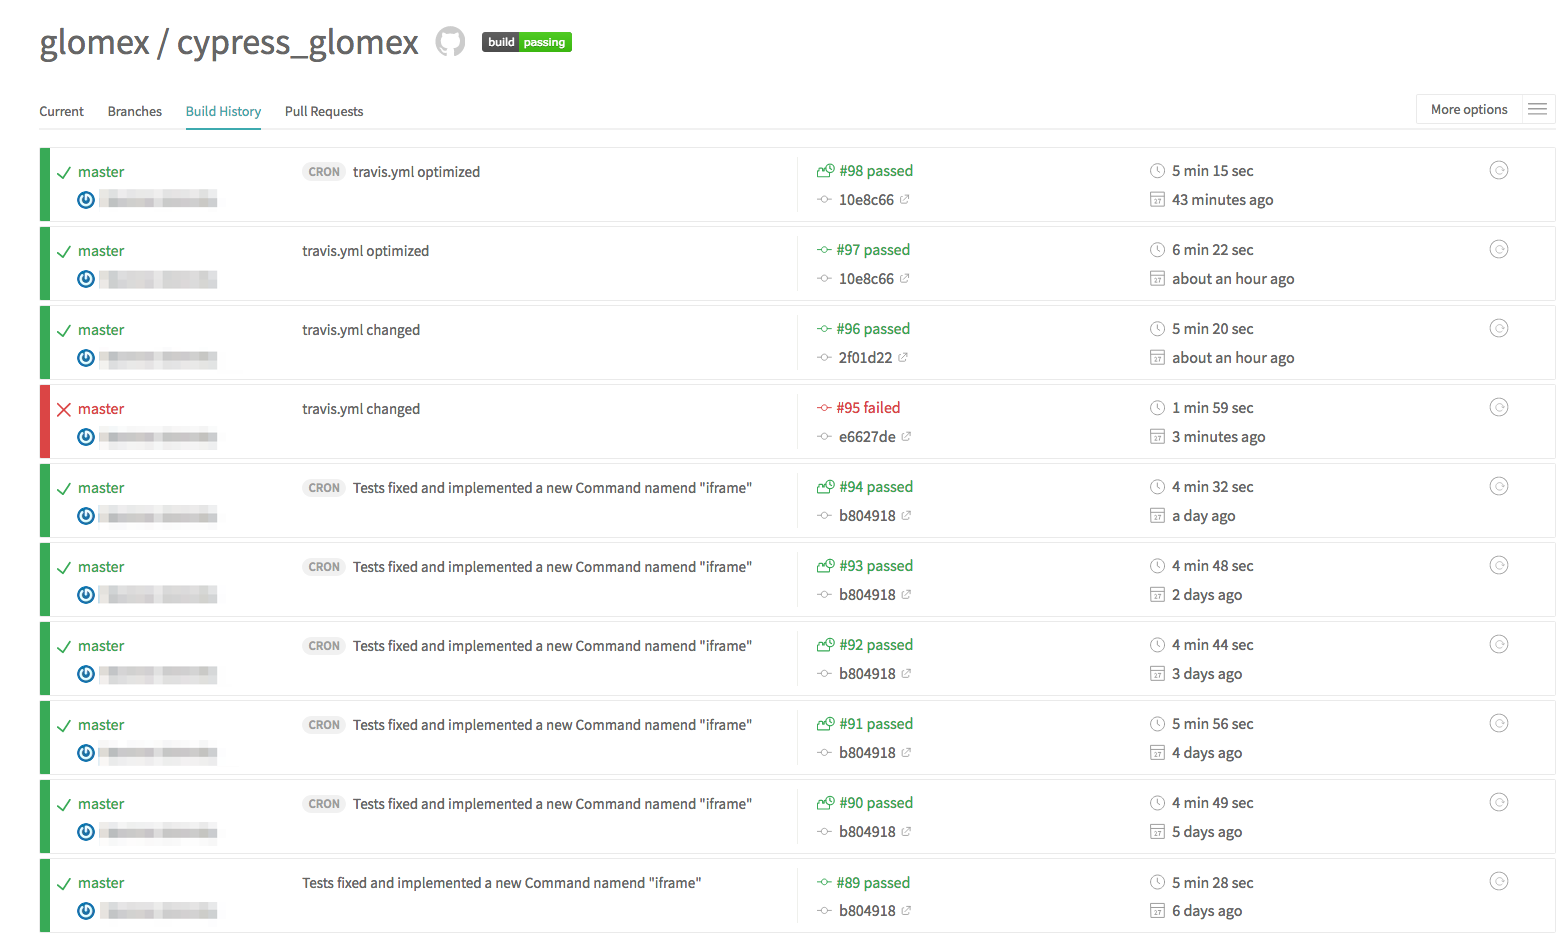
\includegraphics[width=0.95\textwidth]{06_Bilder/travis_tests.png}
	\setlength{\abovecaptionskip}{1em}
	\caption{Travis Testausf�hrung der letzten sechs Tage (Cypress Tests)}
	\label{img:travis_tests}
\end{figure}

\begin{figure}[H]
	\centering
	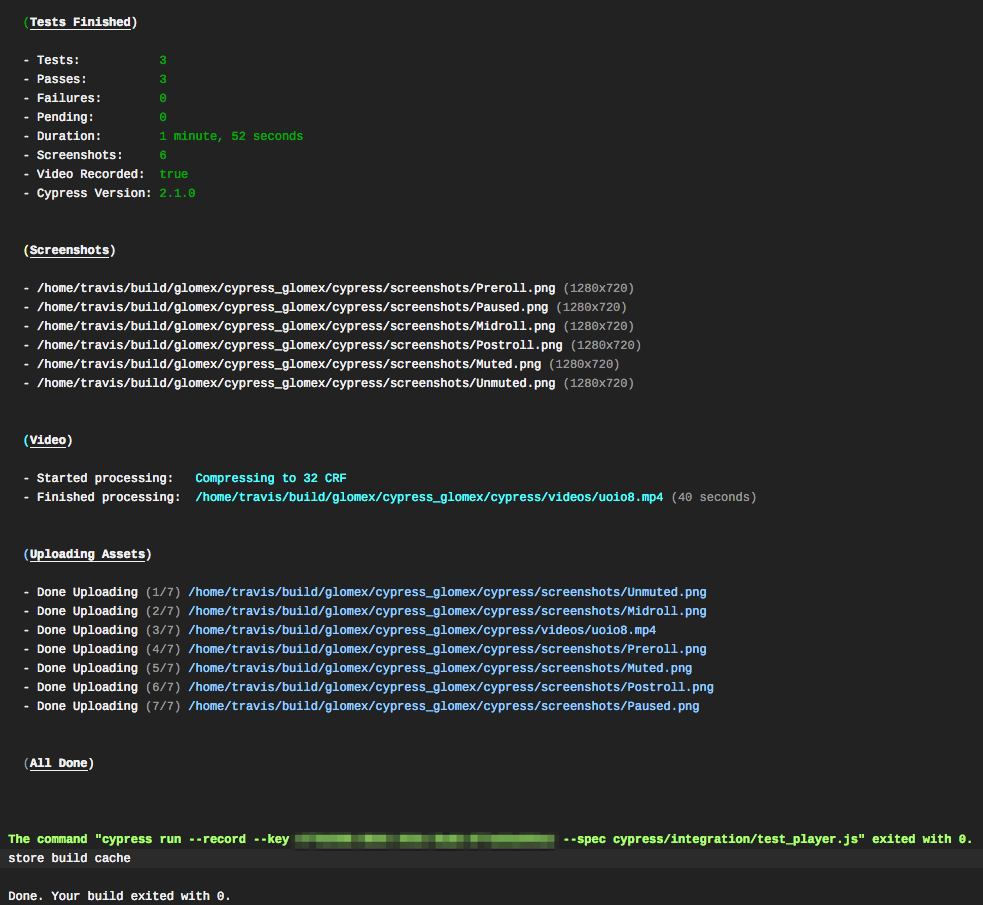
\includegraphics[width=0.9\textwidth]{06_Bilder/travis_log.png}
	\setlength{\abovecaptionskip}{1em}
	\caption{Travis Log nach Abschluss eines Cypress Tests}
	\label{img:travis_log}
\end{figure}

\section{Cypress Dashboard} \label{def:cypress_dashboard}
Cypress bietet ein eigenes Dashboard zur genaueren Analyse automatisierter Tests unter \autocite{cypressDashboard} an. Wie auch bei Travis ist f�r einen Login, ein GitHub Account Voraussetzung.

\begin{figure}[H]
	\centering
	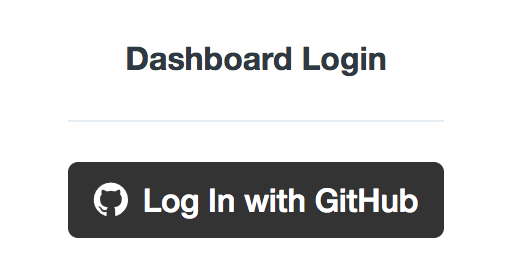
\includegraphics[width=0.7\textwidth]{06_Bilder/dashboard_login.png}
	\setlength{\abovecaptionskip}{0em}
	\caption{Dashboard Login (Quelle: \autocite{cypressDashboardLogin})}
	\label{img:dashboard_login}
\end{figure}

Damit das Dashboard auch Daten zur Auswertung erh�lt, muss es erst verkn�pft werden. Diese Verkn�pfung geschieht durch die Erstellung einer sogenannten \enquote{Project ID}. Um diese zu generieren, muss ein Projekt erstellt und einer Organisation zugeordnet werden. Als Organisation wird die glomex angegeben. Der Projektname l�sst sich frei w�hlen und lautet in diesem Fall \enquote{cypress\_glomex}. Nachdem das Projekt erstellt ist, kann �ber die Einstellungen die sechs stellige Project ID ausgelesen werden. 

\begin{figure}[H]
	\centering
	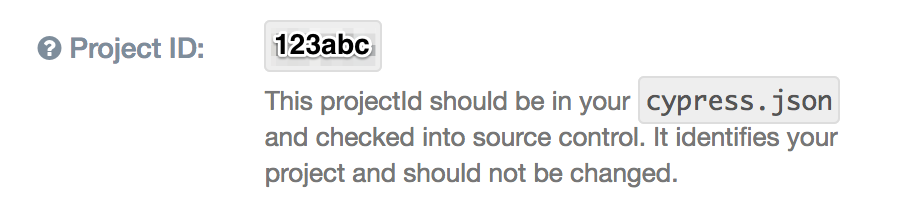
\includegraphics[width=0.7\textwidth]{06_Bilder/dashboard_projectid.png}
	\setlength{\abovecaptionskip}{1em}
	\caption{Project ID (aus Sicherheitsgr�nden hier nur fiktiv)}
	\label{img:dashboard_projectid}
\end{figure}

Cypress gibt an, die Project ID in die \enquote{cypress.json} (siehe Abbildung \ref{img:cypress_folder}) Datei einzutragen und nicht wieder zu ver�ndern (siehe Abbildung \ref{img:dashboard_projectid}). Die Datei muss ebenso in das aktuelle \gls{repository} hochgeladen werden. Anhand der Project ID verkn�pft Cypress w�hrend jeder der Testausf�hrung �ber Travis, den ausgef�hrten Test, mit dem im Dashboard erstellten Projekt. So wird nach jeder Testausf�hrung automatisch jeder Test im Cypress Dashboard angezeigt. 

\begin{figure}[H]
	\centering
	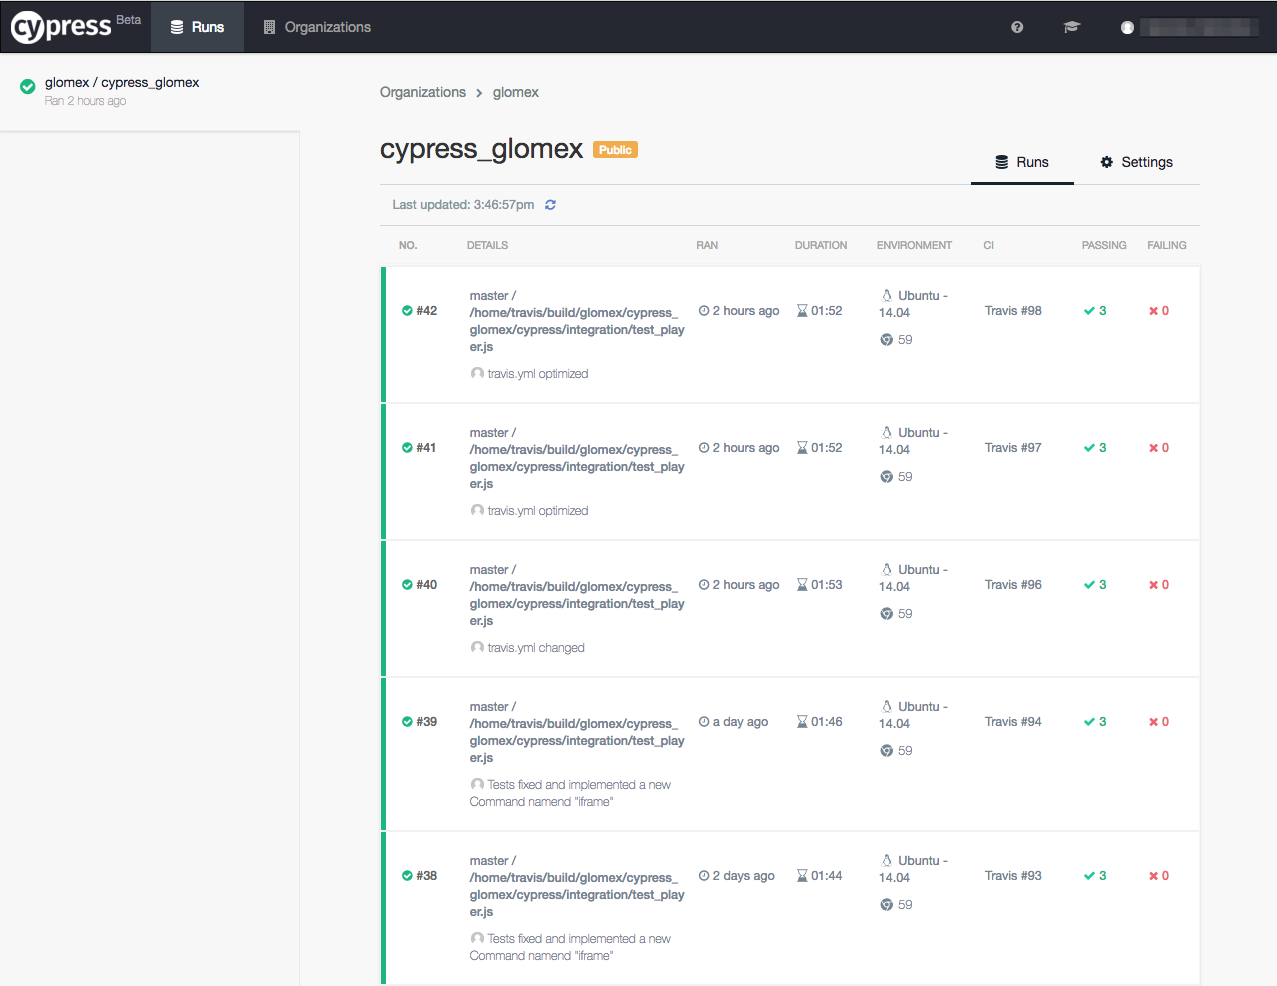
\includegraphics[width=1.0\textwidth]{06_Bilder/dashboard_testausfuehrung.png}
	\setlength{\abovecaptionskip}{0em}
	\caption{Testausf�hrungen im Projekt cypress\_glomex}
	\label{img:dashboard_testausfuehrung}
\end{figure}

\begin{figure}[H]
	\centering
	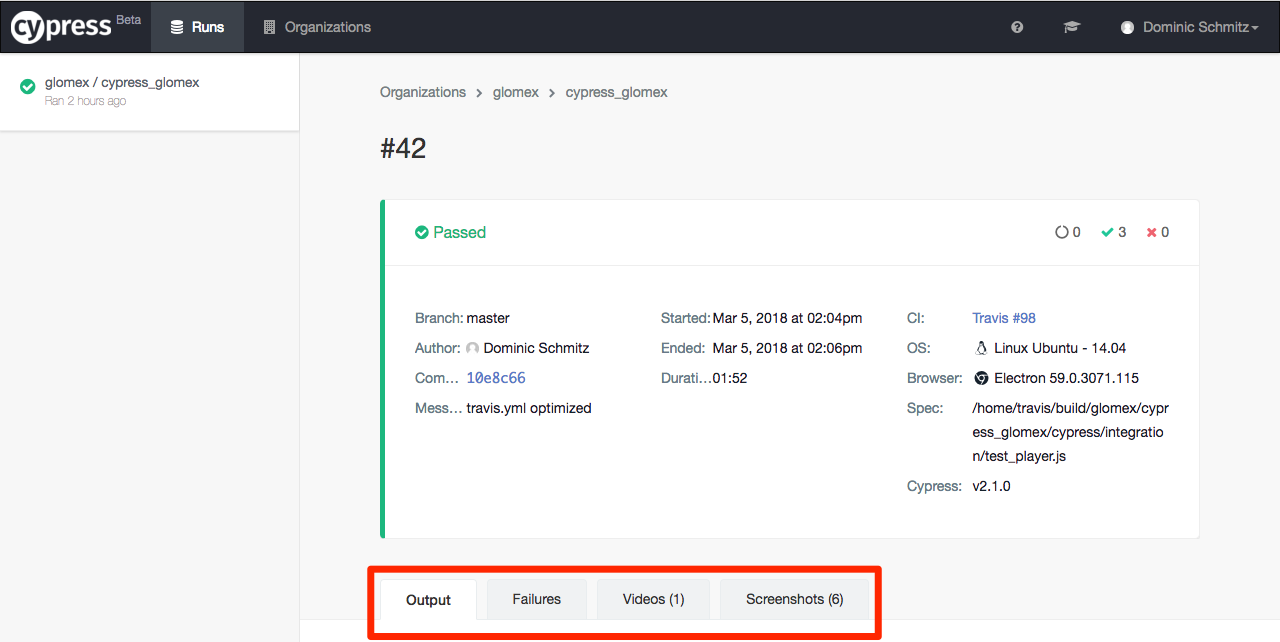
\includegraphics[width=1.0\textwidth]{06_Bilder/dashboard_test_detail.png}
	\setlength{\abovecaptionskip}{0em}
	\caption{Testdetails}
	\label{img:dashboard_test_detail}
\end{figure}

\newpage

Um mehr Daten zur Ausf�hrung eines Tests zu erhalten, kann der jeweilige Test angeklickt werden. Innerhalb des Tests werden genauere Daten wie etwa der auszuf�hrende \gls{branch}, das Start- und Enddatum, die L�nge der Testausf�hrung, das Betriebssystem oder der Browser angezeigt (siehe Abbildung \ref{img:dashboard_test_detail}). Zus�tzlich k�nnen die folgenden Reiter angeklickt werden:

\begin{itemize}
	
	\item \textbf{Output}\\
	In diesem Reiter wird die Ausgabe des Logs angezeigt (siehe Anhang \ref{img:anhang_testdetail_output}).
	
	\item \textbf{Failures}\\
	Sobald ein Fehler aufgetreten ist, wird er unter dem Reiter \enquote{Failures} angezeigt (siehe Anhang \ref{img:anhang_testdetail_failures}).
	
	\item \textbf{Videos}\\
	Wie in Zeile 18 im Codebeispiel \ref{lst:travis.yml} angegeben, wird ein Video des kompletten Testablaufs erstellt. Unter dem Reiter \enquote{Videos} kann dieses Video angesehen werden (siehe Anhang \ref{img:anhang_testdetail_videos}). 
	
	\item \textbf{Screenshots}\\
	Wenn im Code mithilfe des cy.screenshot() Befehls ein Screenshot erstellt wurde, wird dieser im Reiter \enquote{Screenshots} angezeigt (siehe Anhang \ref{img:anhang_testdetail_screenshots}).\\
	
\end{itemize}

Zusammenfassend zeigt sich, dass Cypress auch mit dem Dashboard, Fokus auf Nachvollziehbarkeit und Einfachheit legt. Es ist Cypress gelungen eine perfekte Erg�nzung, zu Travis und dem Cypress Test Runner zu schaffen. Durch die Videoaufnahme und Sicherung der Screenshots kann jederzeit nachvollzogen werden, wo das Problem w�hrend der Ausf�hrung aufgetreten ist. Somit k�nnen auch Probleme ohne jegliche Programmierkenntnisse ermittelt werden, wenn beispielsweise die Webseite nicht erreichbar ist oder das Video nicht abspielt. Das Dashboard ist momentan noch kostenfrei (Stand 05.03.2018). Eine kostenpflichtige Version f�r private \glspl{repository} ist in Planung. 
% !TEX root = Vergleich.tex

\chapter{Vergleich}
Dieses Kapitel soll die wesentlichen Unterschiede des momentan bei der glomex verwendeten Systems Selenium in Verbindung mit Pytest und Python gegen�ber Cypress ermitteln. Anzumerken ist hierbei, dass ausschlie�lich Webplayer Tests f�r diese Arbeit verwendet werden. Anschlie�end sollen diese Unterschiede �bersichtlich und nachvollziehbar dargestellt werden. 

\section{Momentanes System} \label{def:Selenium_momentan}
Wie bereits beschrieben, besteht das momentan eingesetzte System aus einer Mischung zwischen Selenium, Python und Pytest. Hierbei �bernehmen die folgenden Komponenten die folgenden Aufgaben:

\begin{itemize}
	
	\item \textbf{Pytest (siehe Kapitel \ref{def:Pytest})}\\
	Mithilfe von Pytest werden die Tests nachvollziehbar geschrieben.
	
	\item \textbf{Selenium (siehe Kapitel \ref{def:Selenium})}\\
	Selenium erm�glicht es auf Webelemente zuzugreifen und mit ihnen zu interagieren.
	
	\item \textbf{Python}\\
	Python ist eine Programmiersprache und schafft somit die Logik des Tests (Klassen, Methoden, Schleifen etc.).
	
\end{itemize}

\begin{figure}[H]
	\centering
	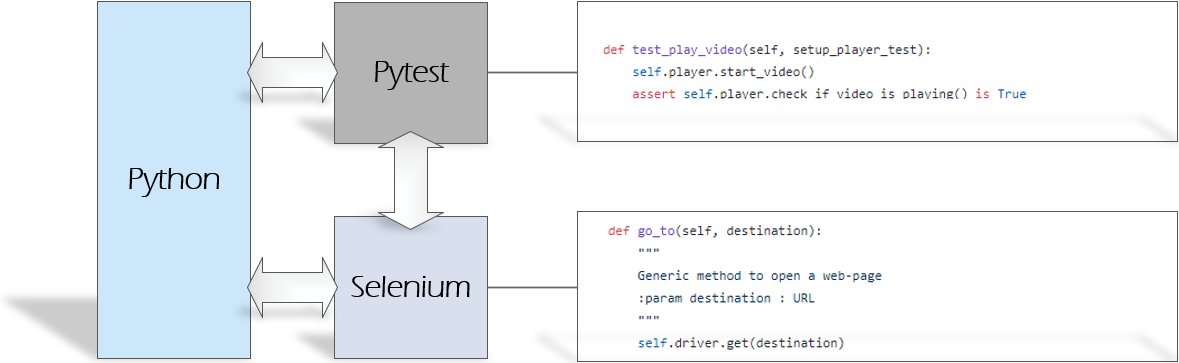
\includegraphics[width=1.0\textwidth]{06_Bilder/Selenium_umgebung.png}
	\setlength{\abovecaptionskip}{1em}
	\caption{Test Umgebung}
	\label{img:selenium_umgebung}
\end{figure}

\newpage
\section{Konzept Vergleich} \label{def:konzept_vergleich}
Beide Frameworks (Selenium und Cypress) verfolgen ein Konzept um Webanwendungen zu testen. Selenium interagiert mithilfe eines Treibers direkt mit dem Browser. Das setzt voraus, dass der jeweilige Treiber des Browsers installiert und konfiguriert ist. Es gibt eine Selenium IDE, mit deren Hilfe es m�glich ist, einzelne Schritte zu automatisieren. Diese ist allerdings nur als \gls{plugin} f�r den Browser Mozilla Firefox erh�ltlich und eher f�r die Erstellung eines einfachen Skripts oder zur Unterst�tzung des explorativen Testens (siehe Kapitel  \ref{def:ExplorativerTest}) gedacht. Um allerdings lokale Tests zu schreiben, die mithilfe eines Servers automatisiert ausgef�hrt werden k�nnen, wird Selenium f�r eine bestimmte Programmiersprache ben�tigt \autocite{seleniumIDE}. 
\\\\
Einen anderen Ansatz versucht Cypress zu realisieren. Cypress Tests werden zwar lokal mithilfe des Cypress Test Runners (siehe Kapitel \ref{def:cypress_test_runner}) gestartet, aber direkt im Browser ausgef�hrt, was dazu f�hrt, dass auch w�hrend der Testausf�hrung auf die Funktionen des Browsers zugegriffen werden kann. Ein weiterer Vorteil ist der geringe Konfigurationsaufwand, da nicht erst ein Treiber installiert und konfiguriert werden muss \autocite{cypress}.
\\\\
Um herauszufinden, welches Konzept sich besser f�r den Einsatz der glomex eignet, wurden verschiedene Kriterien aufgestellt. Die Kriterien wurden aufgrund von Erfahrungen eines sechsmonatigen Praktikums innerhalb der \acs{QA}-Abteilung und der Befragung von \acs{QA}-Mitarbeitern ermittelt. 

\begin{itemize}
	
	\item \textbf{Installation}\\
	Um Tests lokal zu entwickeln und auszuf�hren, wird eine Installation und Konfiguration des jeweiligen Frameworks ben�tigt. Besonders in Unternehmen oder Projekten, bei denen die Fluktuation sehr hoch ist, ist eine einfache, kurze und nachvollziehbare Installation von Relevanz.
	
	\item \textbf{Abh�ngigkeiten}\\
	Jeder Test, der mithilfe eines der Frameworks entwickelt wird, muss ausf�hrbar sein. Die Frage bei diesem Kriterium ist, in wie fern das eingesetzte Framework abh�ngig von weiteren Frameworks, Programmiersprachen und Tools ist, bis sich dieses ausf�hren l�sst. Desto mehr Software vorhanden sein muss, desto h�her ist die Komplexit�t. Das kann dazu f�hren, dass die Ursachen entstandener Fehler aufgrund des zusammenspiels mehrerer Komponenten nur schwer zu identifizieren sind.
	
	\newpage
	
	\item \textbf{Ausf�hrung w�hrend der Testerstellung}\\
	W�hrend der Testerstellung wird ein Test mehrfach wiederholt. Hier stellt sich die Frage, ob das verwendete Framework in Echtzeit �nderungen im Code erkennt und anzeigt, oder bei jeder �nderung der Test nur �ber Umwege ausgef�hrt und �berpr�ft werden kann.
	
	\item \textbf{Kompatibilit�t}\\
	Eines der wichtigsten Kriterien ist die Kompatibilit�t, da Unternehmen wie die glomex darauf angewiesen sind, auf so vielen Plattformen wie M�glich zu testen. Nur so kann gew�hrleistet werden, dass Software weitestgehend fehlerfrei beim Anwender ausgeliefert wird. Im Rahmen dieser Arbeit spielt dabei das sogenannte \gls{crossBrowser} eine Rolle. \gls{crossBrowser} testet eingebetteten Inhalt wie etwa einen Webplayer auf mehreren Browsern, um zu gew�hrleisten, dass dieser sich unabh�ngig vom Browsertyp identisch verh�lt \autocite{crossBrowser}.
	
	\item \textbf{iFrame Support}\\
	Ein weiterer Punkt ist der Support von sogenannten \enquote{iFrames}, auch \enquote{Inlineframes} genannt. Ein \gls{iframe} dient der Strukturierung von Webseiten und stellt weitere Webinhalte als eigenst�ndige Dokumente innerhalb eines definierten Bereichs eines Browsers dar \autocite{iFrame}. Da alle Produkte der glomex \glspl{iframe} zur Darstellung benutzen, ist der Support des Frameworks entsprechend wichtig.
	
\end{itemize}

Jedes der beiden Frameworks wird nun auf das jeweilige Kriterium gepr�ft und verglichen. Dabei erhalten beide Frameworks jeweils eine Punktzahl zwischen 1 (schlecht) bis 3 (gut). Mithilfe dieser vergebenen Punkte wird bei der Auswertung eine Gesamtpunktzahl ermittelt. Mit diesen ist es m�glich, dass f�r die glomex geeignetere Framework zu ermitteln. 

\begin{itemize}
	
	\item \textbf{Installation}\\
	Wie bereits in Kapitel \ref{def:installation} beschrieben ist es m�glich Cypress auf allen g�ngigen Betriebssystemen wie Linux, Mac OS und Windows zu installieren. Cypress bringt mit der Installation alles mit, um Tests zu erstellen und auszuf�hren. Zus�tzlich ben�tigt die Installation kaum Vorwissen und ist auf der Seite \autocite{cypress} nachvollziehbar erl�utert. Die Installation des Cypress Test Runners ist mit wenig Aufwand nach kurzer Zeit abgeschlossen. Ein weiterer positiver Aspekt ist, Cypress warnt sobald eine neuere Version verf�gbar ist und l�sst sich mit nur wenig Aufwand updaten (siehe Kapitel \ref{def:cypress_update}).
	
	\newpage
	
	Selenium unterst�tzt wie auch Cypress alle g�ngigen Betriebssysteme, beinhaltet allerdings nicht alle ben�tigten Komponenten um Tests zu entwickeln. Um Selenium zu nutzen, muss vorher festgelegt werden, in welcher Programmiersprache die Tests sp�ter entwickelt werden. Ist dies geschehen, muss die ben�tigte Programmiersprache, das dazu passende Selenium Paket und der Treiber installiert werden. Anschlie�end muss der Treiber konfiguriert werden \autocite{seleniumInstallation}.
	\\\\
	Der Vergleich zeigt deutlich, das Cypress gro�en Wert auf eine einheitliche, einfache und komplette Installation legt und erh�lt daher 3 Punkte. Bei der Installation von Selenium gestaltet sich die Installation im Vergleich deutlich aufwendiger, da dieser die Installation und Konfiguration mehrerer Komponenten zugrunde liegt, was nur zu einer Bewertung von einem Punkt gef�hrt hat.
	
	\begin{itemize}
		\item Cypress \textbf{3 Punkte}
		\item Selenium \textbf{1 Punkt}\\
	\end{itemize}
	
	\item \textbf{Abh�ngigkeiten}\\
	W�hrend der Installation wird erl�utert, dass Cypress bereits alles an Software mitbringt, um Tests auszuf�hren. Somit werden alle Abh�ngigkeiten durch die Installation beseitigt. Um allerdings Tests komfortabel zu erstellen, wird eine entsprechende \acs{IDE} wie etwa Visual Studio Code angeraten (siehe Kapitel \ref{def:visual_studio}).
	\\\\
	Mindestens eine Programmiersprache wird dagegen von Selenium ben�tigt. In der Realit�t ist das allerdings nicht die einzige Abh�ngigkeit. Selenium alleine f�hrt nur Befehle aus, die an den Browser geschickt werden, um den Browser zu steuern \autocite{selenium}. Aus diesem Grund muss ein entsprechender Treiber f�r jeden Browser, der genutzt werden will, vorhanden und konfiguriert sein. Zus�tzlich werden in der Praxis h�ufig zus�tzlich \acs{BDD}-Frameworks verwendet (siehe Kapitel \ref{def:BDD}), um die Nachvollziehbarkeit eines Tests zu verbessern. 
	\\\\
	Bez�glich der Abh�ngigkeiten hat Cypress einige Vorteile gegen�ber Selenium, da die Hersteller darauf geachtet haben alles an Software das zur Ausf�hrung von Tests ben�tigt wird, direkt mit zu installieren. Da Cypress so gesehen keine Abh�ngigkeiten aufweist, erh�lt das Framework 3 Punkte. Selenium hingegen erh�lt nur einen Punkt, da alleine ohne Konfiguration und Installation weiterer Programmiersprachen und Treiber keine Tests entwickelt werden k�nnen.
	
	\begin{itemize}
		\item Cypress \textbf{3 Punkte}
		\item Selenium \textbf{1 Punkt}\\
	\end{itemize}
	
	\item \textbf{Ausf�hrung w�hrend der Testerstellung}\\
	W�hrend der Testerstellung erm�glicht der Cypress Test Runner einen parallelen Testablauf im Browser. So wird nach jeder �nderung am Quellcode direkt der Test erneut ausgef�hrt und der Entwickler erh�lt Feedback, ob die �nderung die gew�nschte Wirkung erzielt hat. Da zus�tzlich der Cypress Test Runner im Browser l�uft, hat der Entwickler Zugriff auf alle Entwicklerfunktionen die Seitens des Browser zur Verf�gung gestellt werden.
	
	\begin{figure}[H]
		\centering
		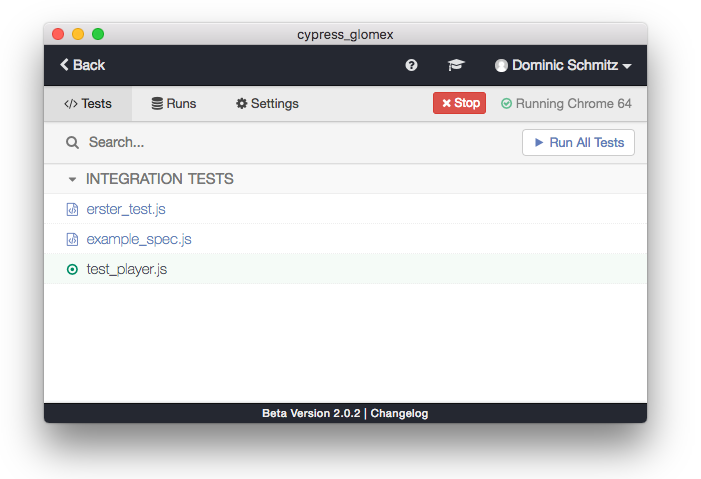
\includegraphics[width=0.8\textwidth]{06_Bilder/cypress_test_runner_running.png}
		\setlength{\abovecaptionskip}{0em}
		\caption{Cypress Test Runner w�hrend der Ausf�hrung des Tests \enquote{test\_player.js}}
		\label{img:cypress_test_runner_running}
	\end{figure}

	\begin{figure}[H]
		\centering
		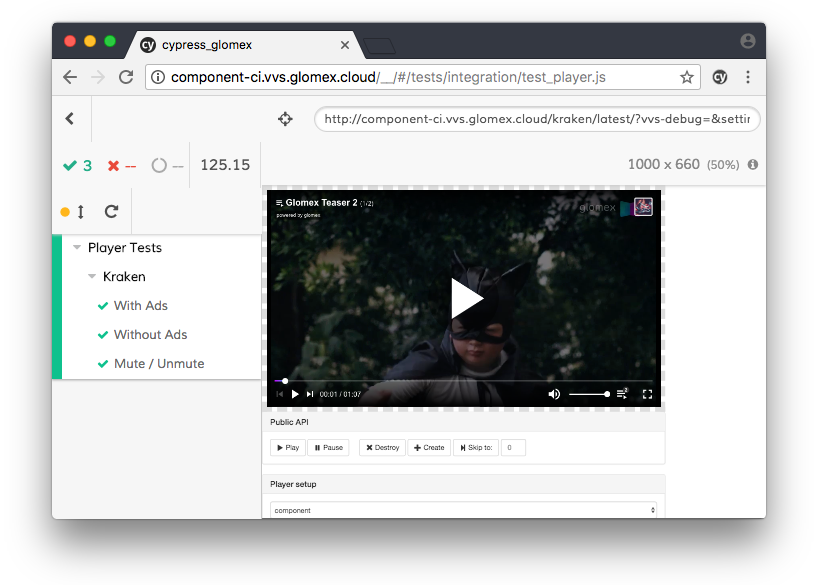
\includegraphics[width=0.8\textwidth]{06_Bilder/cypress_browser_running.png}
		\setlength{\abovecaptionskip}{0em}
		\caption{Testausf�hrung des Tests \enquote{test\_player.js} im Browser Google Chrome}
		\label{img:cypress_browser_running}
	\end{figure}

	Aus dem Grund, das Selenium alleine nicht ausgef�hrt werden kann, wird das momentane System als Referenz verwendet (siehe Kapitel \ref{def:Selenium_momentan}). Bei dem momentanen System wird Selenium mithilfe von Pytest in Verbindung mit der Programmiersprache Python ausgef�hrt. Pytest erkennt keine �nderungen im Code, was dazu f�hrt, dass jeder Test manuell nach jeder �nderung neu gestartet werden muss. Das kann dazu f�hren, dass der Entwickler Fehler �bersieht, da ihm diese nicht direkt angezeigt werden. Da Selenium nur Befehle an den Browser schickt, die anschlie�end ausgef�hrt werden, muss weiterhin eine zus�tzliche Browserinstanz ge�ffnet bleiben, um �ber die Entwicklerkonsole neue Webelemente zu identifizieren.
	\\\\  
	Aufgrund der Komfortabilit�t, Lauff�higkeit im Browser und aktiven Testausf�hrung w�hrend der Entwicklung erh�lt Cypress drei Punkte. Da im Rahmen dieser Arbeit nur das momentane System betrachtet wird und es sehr viele verschiedene Kombinationen der Frameworks gibt, ist nicht ausgeschlossen, dass eine Frameworkkombination (inklusive Selenium) mit einer hohen Komfortabilit�t und aktiven Testausf�hrung existiert. Selenium allerdings kann nicht im Browser ausgef�hrt werden, was zu einer Punktzahl von zwei Punkten f�hrt.
	
	\begin{itemize}
		\item Cypress \textbf{3 Punkte}
		\item Selenium \textbf{2 Punkte}\\
	\end{itemize}
	
	\item \textbf{iFrame Support}\\
	Seitens Cypress gibt es keinen vollen iFrame-Support (stand 27.02.2018). Cypress arbeitet bereits an dem Problem. Intern tr�gt es die Problemnummer 136 (englisch Issue \#136). In der Offiziellen Dokumentation (zu finden unter \autocite{cypressIssue136}) wird folgendes geschrieben:
	\\
	
	\begin{definition}{Zitat aus \autocite{cypressIssue136}}{def:definitionIframeSupport}
		\\ You cannot target elements or interact with anything in an iframe - regardless of it being a same domain or cross domain iframe.\\
		
		This is actively being worked on in Cypress and you'll first see support for same domain iframes, followed by cross domain (they are much harder to do).\\
		
		\textbf{Workaround:}
		
		Sit tight, comment on the issue so we know you care about this support, and be patient.\\
	\end{definition}

	Da die Produkte der glomex iFrames benutzen, muss eine L�sung f�r dieses Problem gefunden werden. Als \gls{workaround} wird empfohlen sich direkt �ber den Github \gls{thread} \autocite{cypressGithubIssue136} an die Entwickler zu wenden. Innerhalb des \glspl{thread} werden bereits einige L�sungsvorschl�ge bereitgestellt, daher ist eine Kontaktaufnahme nicht n�tig. 
	\\\\
	Der in dieser Arbeit verwendete \gls{workaround} sieht vor, einen neuen Befehl zu erstellen (siehe \ref{def:cypress_projektstruktur}, Support). Der erstellte Befehl soll auf ein �bergebenes \gls{iframe} zugreifen und es als eine Referenz zur�ck geben, die dann innerhalb eines Alias gespeichert wird. Ein Alias beschreibt in dieser Arbeit, einen Namen f�r eine Referenz auf ein Objekt.
	
	\lstset{style=cypress, caption={Eigener Befehl \enquote{iframe}}, label={lst:befehl_iframe}}
	\begin{lstlisting}
Cypress.Commands.add('iframe', 
  (locator, element, wait=10000) => {
	  
	return cy.get('iframe',  { timeout: wait })
	  .should('have.class', locator)
	  .should(($iframe) => {
	  	expect($iframe.contents().find(element)).to.exist
	  }).then(($iframe) => {
	  	return cy.wrap($iframe.contents().find("body"))
	  });
		  
})
	\end{lstlisting} 
	
	Wie in Zeile zwei im Codebeispiel \ref{lst:befehl_iframe} dargestellt, werden die folgenden drei Parameter an den Befehl \enquote{iframe} �bergeben:
	
	\begin{itemize}
		\item \textbf{locator}\\
		 Der \gls{locator} der das \gls{iframe} Element eindeutig adressiert. Ein Beispiel hierf�r k�nnte der Klassenname des \glspl{iframe} sein.
		
		\item \textbf{element}\\
		Ein Element innerhalb des \glspl{iframe}, um zu gew�hrleisten, dass auf Elemente innerhalb zugegriffen werden kann.
		
		\item \textbf{wait}\\
		Die Zeit, wie lange gewartet wird, bis das \gls{iframe} Element gefunden werden muss. Standard hier sind 10000 Millisekunden, was 10 Sekunden entspricht. 
		
	\end{itemize}

	\newpage

	Weiterhin ab Zeile vier im Codebeispiel \ref{lst:befehl_iframe} ist zu sehen, dass mithilfe des \enquote{get}-Befehls auf das \gls{iframe} zugegriffen wird. �ber \enquote{should} wird zus�tzlich gepr�ft, ob es sich hierbei um das �bergebene \gls{iframe} handelt. 
	Seit Version 0.20.0 kann mit \glspl{iframe} �ber den \enquote{wrap}-Befehl (siehe Codebeispiel \ref{lst:wrap}) interagiert werden \autocite{cypressChangelog}. Vollst�ndiger Zugriff, damit Cypress innerhalb eines \glspl{iframe} ausgef�hrt werden kann, ist noch nicht m�glich, wird aber in Aussicht gestellt (Stand 27.02.2018). Der eigentliche \gls{workaround} findet in der Zeile sieben (siehe Codebeispiel \ref{lst:befehl_iframe}) statt. Hier wird mit dem wrap-Befehl auf den Content (body) des \glspl{iframe} zugegriffen und anschlie�end zur�ck gegeben. 

	\lstset{style=cypress, caption={erster\_test.js, Quellcode}, label={lst:testausfuehrung}}
\begin{lstlisting}
describe('Player Test', function() {

 beforeEach(function(){
	// Fixtures aus anderen Dateien laden
	cy.fixture('kraken/locators.json').as('locator')
	cy.fixture('kraken/web.json').as('web')
	cy.fixture('kraken/settings.json').as('setting')
 })

 context('Kraken', function(){
   
  it('With Ads', function(){
  
	   // Aufruf der Kraken-Webseite
	  cy.visit(this.web.krakenUrl)
	  
	  // iFrame mit dem Alias "player" (siehe .as(player))
	  cy.iframe(this.locator.playerIframe, "#player")
	    .as('player')
	    
	  // Rufe den Alias mithilfe von ".get" auf, 
	     finde das Webelement und klicke auf Play
	  cy.get("@player").find(this.locator.playButton)
	    .click()
   }) 
  })
})
\end{lstlisting} 

\begin{figure}[H]
	\centering
	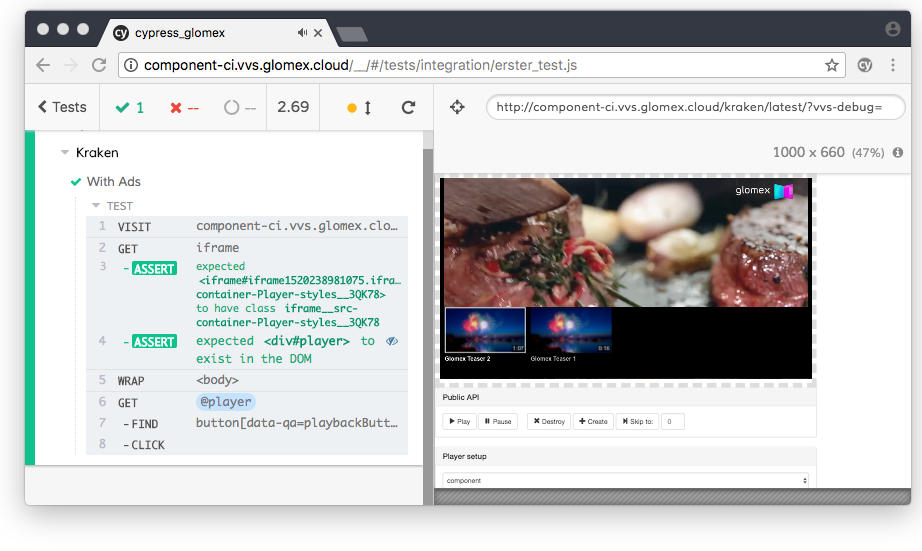
\includegraphics[width=0.95\textwidth]{06_Bilder/cypress_testausfuehrung_browser.png}
	\setlength{\abovecaptionskip}{0em}
	\caption{erster\_test.js, Testausf�hrung im Browser mithilfe des Cypress Test Runners}
	\label{img:cypress_testausfuerung_browser}
\end{figure}

	Codebeispiel \ref{lst:testausfuehrung} zeigt, wie der im Codebeispiel \ref{lst:befehl_iframe} erstellte Befehl angewendet wird. Erst wird mithilfe des \enquote{visit}-Befehls in Zeile 20 auf die Webseite zugegriffen. In Zeile 23 wird der Befehl \enquote{iframe} aufgerufen. W�hrend des Aufrufs wird der \gls{locator} (this.locator.playerIframe) und ein Webelement, das sich innerhalb des \glspl{iframe} befindet (\#player) an den Befehl �bergeben. Dabei ist anzumerken, dass innerhalb eines css Selektors eine Raute auf eine id hinweist. So bedeutet in unserem Beispiel \#player, das der Test nach dem Webelement mit der id \enquote{player} auf der aufgerufenen Webseite suchen soll. Anschlie�end wird mit dem Befehl \enquote{as} ein Alias erstellt. Dieser Alias kann nun weiterhin verwendet werden und repr�sentiert das komplette \gls{iframe} des Players. Zu erw�hnen ist, dass der Alias bis zum ende des it-Blocks bestehen bleibt. 
	\\\\
	In Zeile 27 des Codebeispiels \ref{lst:testausfuehrung} ist sehr gut zu erkennen, dass mithilfe des \enquote{@} Zeichens der Alias, an den get-Befehl �bergeben wird. Folgend kann durch den find-Befehl ein Webelement innerhalb des \glspl{iframe} gesucht und geklickt (.click()) werden. 
	\\\\
	Da es einen \gls{workaround} f�r Cypress gibt mit dessen Hilfe es m�glich ist auf \glspl{iframe} zuzugreifen, erh�lt Cypress f�r dieses Kriterium 2 Punkte. Selenium dagegen supportet \glspl{iframe} vollst�ndig. Der Befehl \enquote{switchTo()} erlaubt es dem Selenium Treiber, direkt das \gls{iframe} aufzurufen und mit ihm zu interagieren. Aus diesem Grund erh�lt Selenium 3 Punkte.

	\begin{itemize}
		\item Cypress \textbf{2 Punkte}
		\item Selenium \textbf{3 Punkte}\\
	\end{itemize}
	
	\item \textbf{Kompatibilit�t}\\
	Das beschriebene \gls{crossBrowser} ist mit Cypress momentan nicht m�glich (siehe Offiziellen Post \autocite{cypressGithubIssue310}), da Cypress nur den Browser \enquote{Google Chrome} (Chrome, Chronium und Canary) unterst�tzt. Die Entwickler stellen aber die Verwendung weiterer Browser in Aussicht (siehe \autocite{cypressGithubIssue310}) f�r zuk�nftige Versionen. Zum  momentanen Zeitpunkt (Stand 27.02.2018) ist dies allerdings nicht m�glich.
	
	\begin{figure}[H]
		\centering
		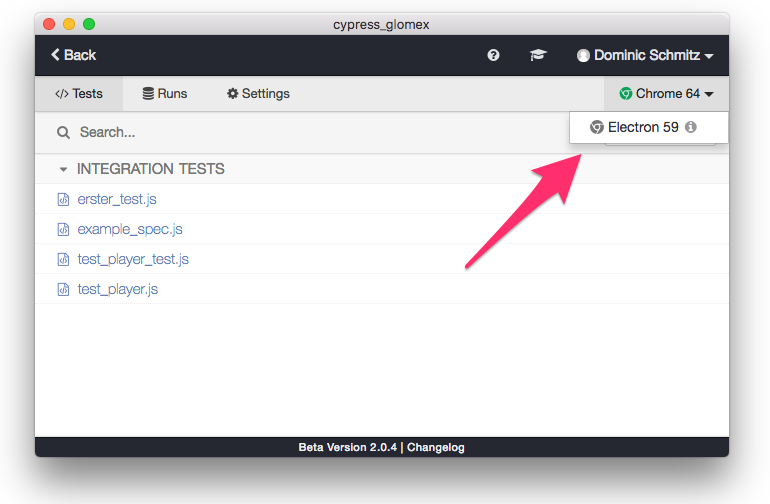
\includegraphics[width=1.0\textwidth]{06_Bilder/cypress_browser.png}
		\setlength{\abovecaptionskip}{-1em}
		\caption{Unterst�tzte Browser im Cypress Test Runner (Stand 27.02.2018 V2.0.4)}
		\label{img:cypress_browser_running}
	\end{figure}

	Offiziell unterst�tzt dagegen Selenium alle g�ngigen Browser wie \enquote{Firefox}, \enquote{Microsoft Internet Explorer}, \enquote{Safari}, \enquote{Opera} und \enquote{Google Chrome}.
	\\\\
	Um ein Webelement anzusprechen, werden bei beiden Frameworks sogenannte \enquote{\gls{locator}s} verwendet. Ein \gls{locator} beschreibt ein HTML Element, beispielsweise mithilfe einer id, eines Klassennamens, weiterer Attribute oder eines Xpaths um dem Framework exakt zu beschreiben, welches Webelement einer Webseite verwendet werden soll. Cypress unterst�tzt derzeit (Stand 22.02.2018) nur css Selektoren um ein Webelement zu beschreiben \autocite{cypress}.
	\\\\
	
	\newpage
	
	Verschiedene Arten unterst�tzt dagegen Selenium. Laut \autocite{seleniumLocators} ist es m�glich �ber folgende Arten ein Webelement zu erreichen:
	
	\begin{itemize}
		\item id
		\item Name
		\item Linktext
		\item Partial Linktext
		\item Tag Name
		\item Class Name
		\item Css
		\item Xpath
	\end{itemize}

	Die genaue Beschreibung jeder M�glichkeit kann auf \autocite{seleniumLocators} nachgelesen werden.
	\\\\
	Das Cypress noch relativ neu im Vergleich zu Selenium ist, wird deutlich im Vergleich der Kompatibilit�t. Besonders da \gls{crossBrowser} seitens Cypress aktuell (Stand 22.02.2018) nicht supported wird, ist es schwer f�r Unternehmen ihre Anwendungen plattform�bergreifend zu Testen. Das ist besonders problematisch, da diese nicht garantieren k�nnen das die Anwendung fehlerfrei beim Anwender funktioniert. Aufgrund dessen erh�lt Cypress im Vergleich nur einen Punkt. Selenium dagegen supported alle g�ngigen Browser und \gls{locator}-Arten, was zu einem Ergebnis von drei Punkten f�hrt. 
	
	\begin{itemize}
		\item Cypress \textbf{1 Punkt}
		\item Selenium \textbf{3 Punkte}\\
	\end{itemize}
	
\end{itemize}

\subsection{Auswertung}

Nachdem alle Kriterien aufgestellt und analysiert wurden, muss nun ausgewertet werden, welches der beiden Frameworks sich besser f�r den Einsatz bei der glomex eignet. Um dies zu ermitteln, wird eine Tabelle mit allen Punkten je Kriterium dargestellt. Die Kriterien Kompatibilit�t und \gls{iframe} Support werden jeweils doppelt gewichtet, da alle Produkte der glomex auf diversen Browsern getestet werden und \glspl{iframe} benutzen.\\

\begin{table}[H]
	\centering
	\begin{tabular}{| l |c|c|c|}
		\hline
		\textbf{Kriterium}    & \textbf{Gewichtung}		& \textbf{Selenium} & \textbf{Cypress} \\ \hline
		Installation          & einfach                 & 1		   & 3		 \\
		Abh�ngigkeiten        & einfach             	& 1		   & 3		 \\
		Ausf�hrung w�hrend der Testerstellung & einfach & 2		   & 3		 \\
		\textbf{Kompatibilit�t}        & \textbf{doppelt}             	& \textbf{6}		   & \textbf{4}		 \\
		\textbf{iFrame Support}        & \textbf{doppelt}             	& \textbf{6}		   & \textbf{2}		 \\ \hline
		Gesamt				  &							& \underline{\underline{\textbf{16}}}	   & \underline{\underline{15}}		 \\ \hline
	\end{tabular}
	
	\caption{Framework Auswertung anhand Kriterien}
	\label{tbl:auswertung}
	
\end{table}

Wie in Tabelle \ref{tbl:auswertung} dargestellt, schneidet Selenium in den Punkten Installation, Abh�ngigkeiten und Ausf�hrung w�hrend der Testerstellung schlecht bis mittelm��ig ab. Das liegt vor allem daran, dass die Installation von Selenium mit diversem Konfigurationsaufwand und der Installation weiterer Frameworks und Programmiersprachen verbunden ist. Ohne eine weitere Programmiersprache kann Selenium nur als Plugin f�r Mozilla Firefox (siehe Selenium IDE \autocite{seleniumIDE}) genutzt werden. \glspl{iframe} unterst�tzt Selenium nativ mithilfe des \enquote{switchTo()} Befehls. Mit ihm ist es m�glich direkt den Fokus des Treibers auf das iFrame zu legen. Selenium funktioniert mit allen g�ngigen Browsern, was sehr von Vorteil ist, da alle Produkte der glomex browserunabh�ngig funktionieren sollen. 
\\\\
Cypress wird st�ndig weiterentwickelt und ist im Gegensatz zu Selenium noch relativ frisch auf dem Markt (Stand 01.03.2018). Die Entwickler legen gro�en Wert auf Komfortabilit�t und �bersichtlichkeit, was sich in der Struktur und Einfachheit der Installation widerspiegelt. Entwickler k�nnen w�hrend der Erstellung und Bearbeitung der Tests genau sehen und nachvollziehen, ob ein Test funktioniert oder nicht, da Cypress nach jeder �nderung den jeweiligen Test erneut ausf�hrt. Der \gls{iframe} Support wurde bereits teilweise umgesetzt (siehe Codebeispiel \ref{lst:befehl_iframe}). Leider fehlt noch eine native L�sung im Bezug auf \glspl{iframe}, um es Cypress direkt zu erm�glichen in das \gls{iframe} zu wechseln und nicht nur mit ihm zu interagieren \autocite{cypressGithubIssue136}. Ein wichtiger Punkt ist zus�tzlich die Kompatibilit�t. Stand 27.02.2018 Version 2.0.4 ist es nicht m�glich einen anderen Browser als Google Chrome f�r Tests zu verwenden \autocite{cypressGithubIssue310}. Es wurde bereits best�tigt das \gls{crossBrowser} zuk�nftig implementiert wird. 
\\\\
Aufgrund der beschriebenen Defizite seitens Cypress ist (Stand 01.03.2018) das momentane System mit 16 (Selenium) gegen�ber 15 (Cypress) Punkten besser f�r den Einsatz bei der glomex geeignet (siehe Tabelle \ref{tbl:auswertung}). Werden in zuk�nftigen Versionen allerdings die M�ngel in Richtung Kompatibilit�t und \gls{iframe} Support behoben, wird Cypress zur deutlich besseren und komfortableren Wahl. 


% !TEX root = Fazit.tex

\chapter{Fazit}

\section{Reflexion} \label{Kap:Reflexion}
Was sind die Ergebnisse dieser Arbeit?

\section{Ausblick} \label{Kap:Ausblick}
Ausblick im Bezug auf die Ergebnisse!

\newpage




% R�mische Ziffern
\roemischenummerierung

% Setze Seitenzahl
\setcounter{page}{13}

% Literatur
\literaturverzeichnis
	
% Anhang
% !TEX root = Anhang.tex

\anhangstart

\phantomsection		
\addstarredchapter{\textbf{Anhang 1, Fragebogen}} % F�gt "Glossar" zum Inhaltsverzeichnis hinzu	
\chapter*{Anhang 1, Fragebogen}

% Abbildung
\begin{figure}[H]
	\centering
	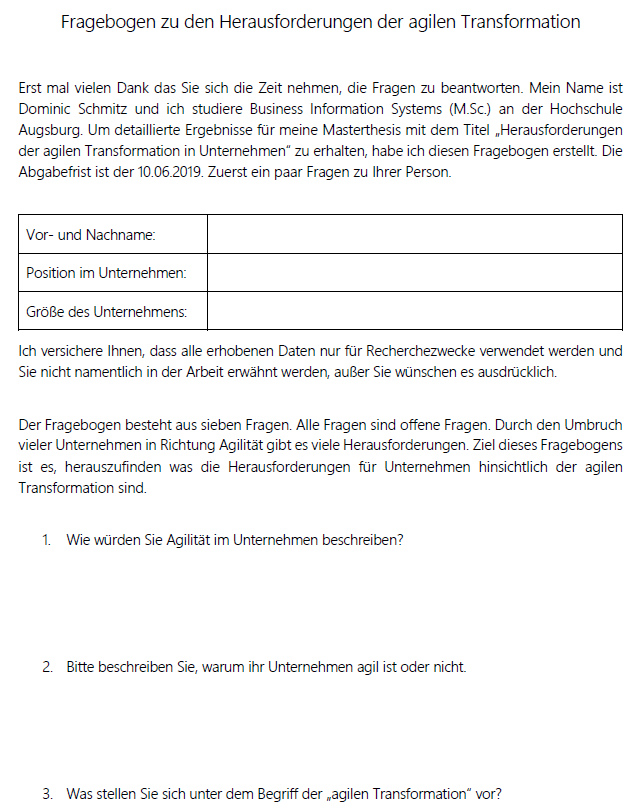
\includegraphics[width=1.0\textwidth]{06_Bilder/Fragebogen_s1.png}
	\setlength{\abovecaptionskip}{1em}
	\caption[]{Fragebogen Seite 1}
	\label{img:anh:fragebogen_s1}
\end{figure}

% Abbildung
\begin{figure}[H]
	\centering
	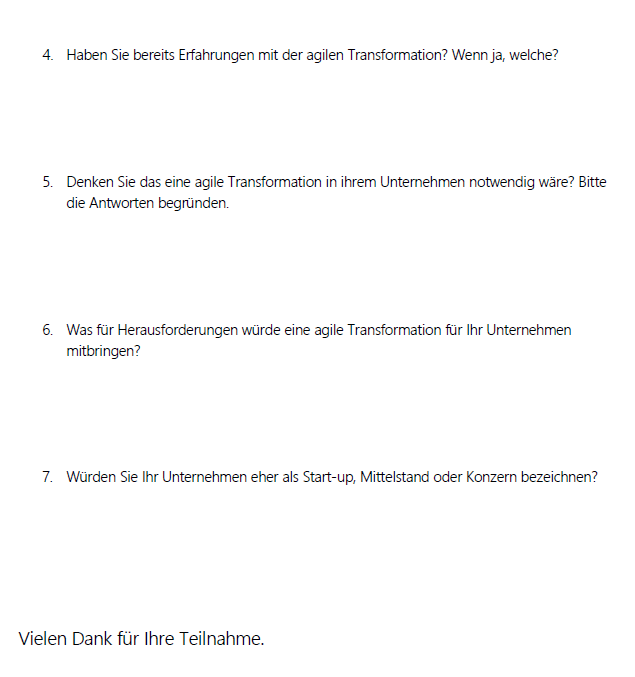
\includegraphics[width=1.0\textwidth]{06_Bilder/Fragebogen_s2.png}
	\setlength{\abovecaptionskip}{1em}
	\caption[]{Fragebogen Seite 2}
	\label{img:anh:fragebogen_s2}
\end{figure}

\phantomsection		
\addstarredchapter{\textbf{Anhang 2, Fragebogen Antworten}} % F�gt "Glossar" zum Inhaltsverzeichnis hinzu	
\chapter*{Anhang 2, Fragebogen Antworten} \label{anh:fragebogen}

\section{Antworten}

\begin{table}[H]
	\centering
	\begin{tabular}{|p{6cm}|p{8cm}|}
		\hline
		\textbf{Position im Unternehmen:}	& Gesch�ftsf�hrer	\\ \hline
		\textbf{Gr��e des Unternehmens:}	& 80 MA 			\\ \hline
	\end{tabular}
	
	\caption{Daten}
	\label{tbl:anh:antw1}
\end{table}

\begin{enumerate}
	\item \textbf{Wie w�rden Sie Agilit�t im Unternehmen beschreiben?}\\
	Agilit�t im Unternehmen bedeutet in erster Linie, dass man als Unternehmen sowie alle Abteilungen und Teams im Einzelnen schnell und unkompliziert auf die sich st�ndig �ndernden �u�eren Faktoren entsprechend reagieren k�nnen. Reagieren hei�t an dieser Stelle nicht \enquote{Dagegenhalten}, sondern diese annehmen und sich m�glichst optimal anpassen oder sogar f�r sich die maximal m�glichen Vorteile daraus ziehen. In agilen Unternehmen h�rt man den Satz \enquote{das haben wir schon immer so gemacht} immer seltener bis gar nicht. Agile Unternehmen sind etwas chaotischer strukturiert, weil nur in einem geordneten Chaos etwas Neues sich formen kann und somit dauerhaft eine Form der Ver�nderung vollzogen wird. 	
	
	\item \textbf{Bitte beschreiben Sie, warum ihr Unternehmen agil ist oder nicht.}\\
	Unser Unternehmen ist agil und soll auch weiterhin agil bleiben. Das Unternehmen geht mit jedem Projekt innovative und zum Teil neue Wege. Mit jedem Projekt, ob es am Ende erfolgreich war oder nicht, gewinnen Mitarbeiter an wertvolle Erfahrung, an neuen Methoden, an neuen Ideen. Es gibt keine feste Teamgrenzen, wir arbeiten vielmehr in virtuellen Teams, die sich auf die Herausforderung jedes Projektes einstellen und neu entstehen. Auch neue Technologien oder neue Methoden werden in unserem Unternehmen nicht nur angenommen, sondern aktiv angewendet und an unsere Kunden weitergegeben. Welche Faktoren sprechen eindeutig daf�r, dass unser Unternehmen agil ist:
	
	\begin{itemize}
		\item Wir haben OKRs eingef�hrt und arbeiten aktiv nach OKR-Modell
		\item Wir haben eine Clean Desk Policy im Unternehmen
		\item Unsere Hierarchien sind sehr flach
		\item Wir sprechen von ?One Team? in dem 80 Mitarbeiter agil arbeiten
		\item Wir erweitern unser Portfolio st�ndig mit neuen Themen
		\item Wir bitten dem Kunden nicht nur das, was wir k�nnen, sondern alles, was wir in der kurzen Zeit vor dem Projektstart noch schaffen zu lernen
		\item Wir haben eine hohe Fehlerkultur, denn nur wer etwas Neues probiert f�llt �fters auf die Nase
		\item Ein GF oder Senior Consultant arbeitet in Projekten auch mit einem Praktikanten zusammen und macht die Sch***-Aufgaben auch alleine 
	\end{itemize}
	
	\item \textbf{Was stellen Sie sich unter dem Begriff der \enquote{agilen Transformation} vor?}\\
	Agile Transformation bedeutet eine dauerhafte Ver�nderung, die sich immer wieder vorsetzt. Eine solche Transformation kann nicht abgeschlossen werden. Sie hat gewisse Etappen, die man erreichen kann, die man auch erreichen muss, aber es geht dann gleich weiter. Es ist eine st�ndige unternehmerische Weiterentwicklung, die gleichzeitig eine Verbesserung ist. Man kann an dieser Stelle sogar von kontinuierlichen Verbesserungsprozessen in einer Organisation sprechen, die zusammengefasst und aus der Flugh�he betrachtet eine agile Transformation des Unternehmens darstellen.
	
	\item \textbf{Haben Sie bereits Erfahrungen mit der agilen Transformation? Wenn ja, welche?}\\
	Fast jeder gr��ere CRM-Ansatz bedeutet eine digitale Transformation, eine neue Art zu arbeiten, mobil zu sein. Solche Projekte werden nicht nur nach agilen Methoden abgearbeitet, sondern legen Grundsteine oder sogar erreichen Etappenziele einer unternehmerischen Transformation. Ob es die gro�e SAFe- oder die kleine SCRUM- Methodik ist, unterscheidet sich die Vorgehensweise im Kern kaum. Mit SAFe wird lediglich die SCRUM-Methodik durch die Skalierung angepasst und sehr breit angewendet. Die Treiber der digitalen Transformation sind in erster Linie die IT-lastige Bereiche eines Unternehmens. F�r die Fachbereiche bedeutet die Transformation gleichzeitig einen Change, daher spielt das Change-Management w�hrend der Transformation eine entscheidende Rolle. Meine Erfahrungen mit der agilen Transformation sind vielseitig, von Neustrukturierung und dadurch Modernisierung der Unternehmensbereiche bis zu IT-Transformation von On-Demand in die Cloud. Dabei arbeiten Gro�konzerne eher nach SAFe-Methodik w�hrend die Mittelst�ndler und Kleinunternehmen von SCRUM sprechen. 
	
	\item \textbf{Denken Sie das eine agile Transformation in ihrem Unternehmen notwendig w�re? Bitte die Antwort begr�nden.}\\
	Ja, diese ist nicht nur notwendig, sondern es ist jedem im Unternehmen Bewusst, dass sich permanent vieles ver�ndern muss, um \enquote{am Ball zu blieben} und dem Mittbewerber immer \enquote{einen Schritt voraus} zu sein. Ob die Ver�nderung in der IT-Landschaft, in der Zusammenarbeit, in der Team-Zusammenstellung oder neue Standorte und neue Themenfelder ? all diese Ver�nderungen geh�ren in unserem Unternehmen zum Alltag und werden von allen Mitarbeitern nicht nur angenommen, sondern auch aktiv mitgestaltet. Wir sind mitten in einer Transformation, mal mehr agil, mal weniger, aber diese Transformation bestimmt unser Arbeitsalltag. Den unsere Kunden erwarten von uns eine Vorbildrolle, was die Digitalisierung angeht, denn wir beraten Sie zu diesen Themen, helfen den Kunden Ihre Herausforderungen in der digitalen Transformation zu schaffen. Denn die Beratungsh�user und Digitale Agenturen sind Pioniere und zugleich die Umsetzer der digitalen Transformation in der Wirtschaft.
	
	\item \textbf{Was f�r Herausforderungen w�rde eine agile Transformation f�r Ihr Unternehmen mitbringen?}\\
	Herausforderungen in folgenden Bereichen:
	\begin{itemize}
		\item \textbf{Interne Organisation:} Durch die stetig wechselnden Projektteams und Themen�berschneidungen ist es schwierig eine interne Organisation so zu fixieren, dass diese zumindest 1-2 Jahre gleich bleibt. Die Herausforderung ist dabei, nach Au�en eine klare Struktur zu zeigen und nach ihnen diese in den Griff zu bekommen ohne klare Grenzen ziehen zu m�ssen.
		
		\item \textbf{Technische Vielfalt:} Die Transformation bring viele technische Tools mit sich, die sinnvoll sind und Mehrwert liefern. Dabei muss man sehr stark aufpassen, dass man sich nicht nur noch mit der Technik besch�ftigt, die einen �berrollt und bereits morgen immer veraltet sein wird egal wie neu diese heute ist. Denn die Transformation bedeutet nicht nur technische Ver�nderung, sondern vielmehr neue Wege gehen, sich immer wieder neu ausrichten, st�ndiges Change Management zu betreiben, neue Methoden auszuprobieren, diese zu Optimieren und neue zu erfinden. Die Technik ist nur Zweck zum Erreichen des Ziels. 
		
		\item \textbf{Den Fokus zu behalten:} Mit st�ndiger Ver�nderung und Neuerung kommt die Gefahr, dass man den Fokus verliert, dass man vergisst, warum man auf dem Markt ist, warum man diese Firma gegr�ndet hat und was man mit der Firma vorhat. Man sollte die gro�en Trends beobachten, sich damit besch�ftigen, aber nicht das gesamte Gesch�ft darauf fokussieren.
		
		\item \textbf{Strategisch zu denken und eine Vision zu haben:} Herausforderung ist dabei, nicht aktionistisch zu handeln, weil es schnell sein muss, sondern strategisch �berlegt. 
		
		\item \textbf{Passende Mitarbeiter zu finden:} Denn nicht jeder mag eine st�ndige Ver�nderung, eine schnelle Entwicklung, Agilit�t in der Arbeit, Vorreiter zu sein. Ein gro�er Teil der in Frage kommenden Mitarbeiter w�rde zwar gerne mitmachen und findet Agilit�t super, aber wenn es dann darauf ankommt, will man 9to5-Job haben und einen festen Arbeitsplatz mit dem Bildrahmen der eigenen Katze auf dem Tisch. Das ist nicht agil, es ist keine Transformation. Das ist SIEMENS-Style bzw. Beamten-Style. 
		
	\end{itemize}
	
	\item \textbf{W�rden Sie Ihr Unternehmen eher als Start-up, Mittelstand oder Konzern bezeichnen?}\\
	Ich w�rde unser Unternehmen noch als Start-up bezeichnen, der auf einem guten Weg zu einem soliden Mittelstand ist. 

\end{enumerate}

\newpage

\section{Antworten}

\begin{table}[H]
	\centering
	\begin{tabular}{|p{6cm}|p{8cm}|}
		\hline
		\textbf{Position im Unternehmen:}	& Spezialist Test Management	\\ \hline
		\textbf{Gr��e des Unternehmens:}	& 200 MA 			\\ \hline
	\end{tabular}
	
	\caption{Daten}
	\label{tbl:anh:antw2}
\end{table}

\begin{enumerate}
	\item \textbf{Wie w�rden Sie Agilit�t im Unternehmen beschreiben?}\\
	Agilit�t bedeutet Verantwortung f�r das eigene Handeln zu �bernehmen sowie Freir�ume und Flexibilit�t f�r die L�sung von Problemstellungen so zu nutzen, dass das bestm�gliche Ergebnis f�r das Unternehmen entsteht.	
	
	\item \textbf{Bitte beschreiben Sie, warum ihr Unternehmen agil ist oder nicht.}\\ 
	Mein Unternehmen ist intern bereits sehr agil, da flache Hierarchien bestehen. Au�erdem sind Teams vorhanden, die nach Scrum und Kanban arbeiten sowie Konfliktmanagementprozesse, die es auf verschiedenen Stufen erm�glichen, Konflikte mit neutralen Kollegen in 1:1 Gespr�chen oder im Team zu l�sen. Dar�ber hinaus kann sich jeder einzelne Kollege einbringen und wird auch geh�rt. In der Zusammenarbeit mit externen Partnern sind wir weniger agil unterwegs, da viele externe Kollegen sehr an Hierarchien glauben und nicht selber Verantwortung f�r das eigene Handeln �bernehmen wollen. Hier ist noch die Denke vertreten: \enquote{Ich mache das, was man mir sagt, dann bekomme ich mein Geld}. Wir versuchen die Leute nun nach und nach weiter zu entwickeln, um auch da wirklich agil zu werde.
	
	\item \textbf{Was stellen Sie sich unter dem Begriff der \enquote{agilen Transformation} vor?}\\
	Agile Transformation ist f�r mich der Weg von einem hierarchischen Betriebsmodell hin zu einem agilen Unternehmen. Dieser Weg ist f�r jedes Unternehmen individuell und muss entsprechend geplant werden, damit alle Mitarbeiter abgeholt werden k�nnen.
	
	\item \textbf{Haben Sie bereits Erfahrungen mit der agilen Transformation? Wenn ja, welche?}\\
	Ja, habe ich. In verschiedenen Unternehmen war ich bei der Planung von Workshops beteiligt oder habe als QA, PO und Scrum Master agile Teams mit aufgebaut. Die Transformationen waren nicht immer leicht, da es besonders darauf ankommt Kollegen zu haben, die offen f�r die Transformation sind. Verschlie�t sich jemand, ist es oftmals unm�glich die Leute zu �berzeugen und sie verlassen �ber kurz oder lang das Unternehmen.
	
	\newpage
	\item \textbf{Denken Sie das eine agile Transformation in ihrem Unternehmen notwendig w�re? Bitte die Antwort begr�nden.}\\
	Die Transformation ist bei uns in Gange und wird auch nie abgeschlossen sein, da man sich immer weiterentwickeln und verbessern kann.
	
	\item \textbf{Was f�r Herausforderungen w�rde eine agile Transformation f�r Ihr Unternehmen mitbringen?}\\
	\begin{itemize}
		\item Externe Mitarbeiter mit eingliedern 
		\item Gegner �berzeugen
		\item Mitarbeiter enabeln Verantwortung zu �bernehmen 
		\item Zusammenarbeit mit dem Mutterkonzern, der noch sehr nach Wasserfall-lastig arbeitet
	\end{itemize}
	
	\item \textbf{W�rden Sie Ihr Unternehmen eher als Start-up, Mittelstand oder Konzern bezeichnen?}\\
	Wir sind der agile Part eines Konzerns
	
\end{enumerate}

\newpage

\section{Antworten}

\begin{table}[H]
	\centering
	\begin{tabular}{|p{6cm}|p{8cm}|}
		\hline
		\textbf{Position im Unternehmen:}	& 	VP Product Strategy\\ \hline
		\textbf{Gr��e des Unternehmens:}	& 	50 MA		\\ \hline
	\end{tabular}
	
	\caption{Daten}
	\label{tbl:anh:antw3}
\end{table}

\begin{enumerate}
	\item \textbf{Wie w�rden Sie Agilit�t im Unternehmen beschreiben?}\\
	\enquote{Agile} geht Hand in Hand mit anderen Konzepten wie \enquote{Lean} und \enquote{Management 3.0}. In meinen Augen ist es vor allem ein Wertesystem und ein Werkzeugkasten. Die Werte sind den Anforderungen einer modernen, digitalen Arbeits- und Gesch�ftswelt angepasst. Aus dem Werkzeugkasten kann man sich bedienen um eine f�r das eigene Unternehmen passenden L�sung zu schaffen. Agilit�t besteht nicht nur aus Prozessen und Workflows, die man kopieren/lernen kann.
	\\\\
	Agilit�t bottom-up einzuf�hren funktioniert aus meiner Erfahrung nicht ? top-down aber auch nicht, wenn das Executive-Management glaubt, dass das ohne Ver�nderungen f�r sie selber m�glich ist oder nicht an die zugrunde liegenden Werte  und Benefits glaubt.
	\\\\
	Es gibt kein Blueprint, es gibt nicht sowas wie \enquote{das Spotify-Modell}. Man kann \enquote{Agilit�t} einem Unternehmen nicht \enquote{verordnen}, durch Consultants beibringen. Man committet sich auf die Werte ? durch alle Managementlevel - und kann sich Unterst�tzung holen den Werkzeugkasten richtig einzusetzen.
	\\\\
	Der Gedanke vom \enquote{lernenden Unternehmen}, das sich permanent weiterentwickelt und der Ver�nderungen anpasst, wird sehr oft au�en vor gelassen/vergessen.
	\\\\
	Agilit�t betrifft alle Aspekte eines Unternehmens ? von der Organisationsstruktur bis zum Zielsystem. Sie ist nichts, was nur \enquote{in der Technik} oder ausschlie�lich in Entwicklungsteams stattfindet. Transformationen, die nur eine Abteilung im Unternehmen betreffen, scheitern schnell.
	\\\\
	Agilit�t wird auch gerne mit \enquote{chaotisch} oder \enquote{ich darf doch als Manager jeden Tag meine Meinung �ndern, oder?} verwechselt.
	\\\\
	Ein sehr h�ufiges Problem ist auch der verbliebene Wunsch nach langfristiger Milestone-Planung, der mit Agilit�t nicht vereinbar ist bzw. den die Agile Welt als nicht sinnvoll darstellt.
		
	
	\item \textbf{Bitte beschreiben Sie, warum ihr Unternehmen agil ist oder nicht.}\\
	Die Bandbreite ist hoch: einzelne Teams arbeiten agiler als andere. Einige Elemente aus dem agilen Werkzeugkasten sind umgesetzt ? aber viele auch nicht. Agile wird nicht durch das gesamte Unternehmen und alle Hierarchieebenen gelebt. Die dem \enquote{Agile} Gedanken zugrundeliegende Werte und Benefits werden aber auch nicht vollst�ndig als valide gesehen.
	\\\\
	Bei Einzelpersonen gibt es auch eine gewisse \enquote{Agile M�digkeit}: Ver�nderungsversuche aus der Vergangenheit, die nicht erfolgreich waren (aus unterschiedlichen Gr�nden), werden der Grundidee angelastet ? dadurch wird zu Weile eher polemisch �ber \enquote{Agile} gesprochen, vor allem im Senior/Executive Management (die klassischer Weise den meisten \enquote{Machtverlust} erleiden, wenn man ein Unternehmen voll und ganz Agile f�hren will).
	\\\\
	Insgesamt ist die Agilit�t f�r ein konzern-nahes Unternehmen vermutlich gar nicht so schlecht, aber gemessen an Digital Champions oder Start-ups sehr bescheiden. Das liegt IMHO vor allem daran, dass das Management nicht an die Ideen und Werte glaubt ? oder nicht bereit ist in die Transformation zu investieren bzw. den damit verbundenen Machtverlust zu akzeptieren.
	
	\item \textbf{Was stellen Sie sich unter dem Begriff der \enquote{agilen Transformation} vor?}\\
	Ich mag den Begriff nicht sehr. F�r mich schwingt da mit, dass man die Mitarbeiter umformt und sie dann nach Projektabschluss am Ziel sind.
	\\\\
	Die Werkzeuge der Agile Community entwickeln sind permanent weiter.
	Ohne mich zu sehr wiederholen zu wollen: man sollte sich auf die Werte committen und die Weichen stellen ein lernendes Unternehmen zu werden ? dann kann man eigentlich dauerhaft die notwendigen Ver�nderungen vornehmen, ohne das man jemals komplett am Ziel ist. Ver�nderung als Dauerzustand.
	
	\item \textbf{Haben Sie bereits Erfahrungen mit der agilen Transformation? Wenn ja, welche?}\\
	Ja, viele. Von Ans�tzen auf der Teamebene, der Abteilungsebene (beides bottom-up), bis zur unternehmensweiten Mission. Wenige allerdings mit nachhaltigen und guten Erfolgen. Zumeist ist es an den Dingen gescheitert, die ich bereits in den vorherigen Antwortet erw�hnt habe.
	\\\\
	Zwischenzeitlich war ich sogar hauptverantwortlich (\enquote{Chief Agile Coach}) f�r die agile Unternehmenskultur und Ver�nderung. Obwohl ich sehr leidenschaftlich an manche der agilen Ideen glaube, habe ich diese Aufgabe am Ende abgegeben ? weil es einfach zu frustierend war in der Umsetzung. Ich habe mir auch vorgenommen ? obwohl ich in dem Bereich einige Erfahrung habe ? nur dann noch mal in einer �hnlichen Rolle in einem anderen Unternehmen t�tig zu werden, wenn ich 100\% davon �berzeugt bin, dass die Unternehmensf�hrung die Konzepte versteht und hinter den Werten steht.
	
	\item \textbf{Denken Sie das eine agile Transformation in ihrem Unternehmen notwendig w�re? Bitte die Antwort begr�nden.}\\
	Ja, ich glaube nach wie vor daran, dass das Unternehmen von mehr \enquote{richtiger} Agilit�t profitieren w�rde: bessere Zusammenarbeit �ber alle Abteilungen, mehr Transparenz; mehr F�higkeit schnell auf den Markt zu reagieren; Ideen schneller austesten und verwerfen, wenn sie nicht genug Potential beweisen, ...
	
	\item \textbf{Was f�r Herausforderungen w�rde eine agile Transformation f�r Ihr Unternehmen mitbringen?}\\
	\begin{itemize}
		\item Nachdem wir in einen Konzern eingebettet sind: Strukturen au�erhalb des Unternehmens, an den Schnittpunkten zum (nicht-agilen) Konzern kompatible zur eigenen Agilit�t machen
		\item Lehre und �berzeugungsarbeit im Senior-Management (Machtverlust kompensieren/akzeptieren)
		\item Wir sitzen an zwei Standorten, bei dem einer auch noch in einem anderen Kulturkreis ist (Ukraine); alle Mitarbeiter mitzunehmen, die agilen Werte zu vermitteln, ist eine nicht zu untersch�tzende Herausforderung
		\item Das Investment der Transformation und die damit verbundenen kurzfristigen Abstriche in der Produktivit�t zu Gunsten der mittel- bis langfristigen Vorteile akzeptieren
	\end{itemize}
	
	\item \textbf{W�rden Sie Ihr Unternehmen eher als Start-up, Mittelstand oder Konzern bezeichnen?}\\
	Hybrid: Start-up like (�hnliche Herausforderungen, partiell Autonomie eines Start-ups), aber eng eingebettet in einen Konzern; Mitarbeiter-Struktur, HR-Themen sind sehr Konzern-nah.
	
\end{enumerate}

\newpage

\section{Antworten}

\begin{table}[H]
	\centering
	\begin{tabular}{|p{6cm}|p{8cm}|}
		\hline
		\textbf{Position im Unternehmen:}	& 	\\ \hline
		\textbf{Gr��e des Unternehmens:}	& 			\\ \hline
	\end{tabular}
	
	\caption{Daten}
	\label{tbl:anh:antw4}
\end{table}

\begin{enumerate}
	\item \textbf{Wie w�rden Sie Agilit�t im Unternehmen beschreiben?}\\	
	
	\item \textbf{Bitte beschreiben Sie, warum ihr Unternehmen agil ist oder nicht.}\\ 
	
	\item \textbf{Was stellen Sie sich unter dem Begriff der \enquote{agilen Transformation} vor?}\\
	
	\item \textbf{Haben Sie bereits Erfahrungen mit der agilen Transformation? Wenn ja, welche?}\\
	
	\item \textbf{Denken Sie das eine agile Transformation in ihrem Unternehmen notwendig w�re? Bitte die Antwort begr�nden.}\\
	
	\item \textbf{Was f�r Herausforderungen w�rde eine agile Transformation f�r Ihr Unternehmen mitbringen?}\\
	
	\item \textbf{W�rden Sie Ihr Unternehmen eher als Start-up, Mittelstand oder Konzern bezeichnen?}\\
	
\end{enumerate}

\newpage

\section{Antworten}

\begin{table}[H]
	\centering
	\begin{tabular}{|p{6cm}|p{8cm}|}
		\hline
		\textbf{Position im Unternehmen:}	& 	\\ \hline
		\textbf{Gr��e des Unternehmens:}	& 			\\ \hline
	\end{tabular}
	
	\caption{Daten}
	\label{tbl:anh:antw5}
\end{table}

\begin{enumerate}
	\item \textbf{Wie w�rden Sie Agilit�t im Unternehmen beschreiben?}\\	
	
	\item \textbf{Bitte beschreiben Sie, warum ihr Unternehmen agil ist oder nicht.}\\ 
	
	\item \textbf{Was stellen Sie sich unter dem Begriff der \enquote{agilen Transformation} vor?}\\
	
	\item \textbf{Haben Sie bereits Erfahrungen mit der agilen Transformation? Wenn ja, welche?}\\
	
	\item \textbf{Denken Sie das eine agile Transformation in ihrem Unternehmen notwendig w�re? Bitte die Antwort begr�nden.}\\
	
	\item \textbf{Was f�r Herausforderungen w�rde eine agile Transformation f�r Ihr Unternehmen mitbringen?}\\
	
	\item \textbf{W�rden Sie Ihr Unternehmen eher als Start-up, Mittelstand oder Konzern bezeichnen?}\\
	
\end{enumerate}

\chapter*{Anhang 3, Interviews}

\textbf{Anmerkung: } Die hier aufgef�hrten Interviews wurden am 06.06.2019 gef�hrt. Die Befragung wurde von Herrn Dominic Schmitz (Autor dieser Arbeit) gef�hrt. Die komplette Befragung wird als .mp3 Datei, dieser Arbeit zugegeben. Folgend wird das gesprochene Wort in Text umgewandelt. Hierbei ist wichtig zu erw�hnen, dass grammatikalische Fehler im besten gewissen verbessert wurden. Dabei wird in keiner wei�e die Bedeutung des Satzes und dessen Informationen ver�ndert. Die hierbei verwendeten Fragen, beziehen sich grundlegend auf die, des Fragebogens aus Anhang \ref{anh:fragebogen}. Es kommt vor, dass zus�tzliche Fragen bez�glich einer Antwort gestellt wurden.

\section{Interview Caroline Wicks Schmitz}

\begin{table}[H]
	\centering
	\begin{tabular}{|p{6cm}|p{8cm}|}
		\hline
		\textbf{Vorname, Nachname:} 		& 	Caroline, Wicks Schmitz			\\ \hline
		\textbf{Position im Unternehmen:}	& 	Chief Financial Officer (CFO)	\\ \hline
		\textbf{Name des Unternehmens:} 	&	C. \& E. Fein GmbH				\\ \hline 
		\textbf{Gr��e des Unternehmens:}	&	ca. 950 MA / 750 Mio. Umsatz im Jahr\\ \hline
	\end{tabular}
	
	\caption{Daten}
	\label{tbl:anh:int1}
\end{table}

\begin{itemize}
	\item \textbf{Wie lautet ihr vollst�ndiger Name?}\\
	Ich hei�e Caroline Wicks Schmitz. Ich bin derzeit CFO (Chief Financial Officer) der Fein Gruppe. Das ist ein Unternehmen mit weltweit circa 950 Mitarbeiternc und einem Jahresumsatz von circa 170 Millionen Euro. 
	
	\item \textbf{Sie willigen ein, dass die Befragung und die hier erhobenen Daten f�r diese Masterthesis verwendet werden d�rfen?}\\
	Selbstverst�ndlich willige ich ein.
	
	\item \textbf{Wie w�rden Sie Agilit�t im Unternehmen beschreiben?}\\
	Grunds�tzlich ist Agilit�t f�r mich eine Methode der Projektverfolgung, die Bewegung und Innovation im Unternehmen f�rdert, im Gegensatz zum klassischen Projektmanagement, dass eher einen starren Ablauf vordefiniert. Bei Fein w�rde ich sagen, dass eher das klassische Projektmanagement verwendet wird. Es werden Meilensteine definiert die den Zielen der Sprints aus agilen Formen �hneln. Zus�tzlich wird auch eine Zielplanung durchgef�hrt und es gibt review Meetings, die nicht t�glich abgehalten werden, sondern im klassischen Sinne nach erreichen eines Meilensteins. F�r die Firma Fein sind die Produktentwicklungsprojekte sehr wichtig im Projektmanagement. Dort gibt es wirklich diesen klassisch definierten Ablauf, wie ein Produkt definiert wird. Ich denke das vielleicht eine agile Vorgehensweise in diesem Bereich mehr Innovation und Kreativit�t fordern k�nnte.
	
	\item \textbf{Sie w�rden also ihren momentanen Prozess als Iterativ bezeichnen, aber die agilen Methodiken w�ren dann doch zukunftstr�chtiger?}
	Ich denke schon, dass da etwas zu gewinnen w�re. In einer klassischen Projektentwicklungsform, gehen die Ingenieure nur Schritt f�r Schritt vor hacken ihre Listen ab. In diesem Bereich w�rde nat�rlich diese reaktive Form der Agilit�t helfen selbst�ndiges Mitdenken, Kreativit�t und Eigeninitiative zu f�rdern.
	
	\item \textbf{Bitte beschreiben Sie, warum ihr Unternehmen agil ist oder nicht.}\\ 
	Ich w�rde Fein nicht als agil beschreiben, weil man eher von oben herab dieses Management by Command and Control hat. Dadurch haben die Mitarbeiter nicht den Mut Entscheidungen selber zu treffen. Das hat zur Folge, dass die Entscheidungsfreiheit und Motivation verloren geht. Die Mitarbeiter haben auch Angst vor offenen Feedback. Oft wird der Hinweis auf Fehler noch missverstanden, da die Mitarbeiter in der Unternehmenskultur noch nicht in der Lage sind, die Vorteile von offenem Feedback zu erkennen. Zus�tzlich wirkt das normale Tagesgesch�ft dagegen. Ich denke jeder Mitarbeiter hat einen hohen Anteil an Tagesgesch�ft und die Bereichs�bergreifende Zusammenarbeit wird dadurch nicht erleichtert.
	
	\item \textbf{Was stellen Sie sich unter dem Begriff der \enquote{agilen Transformation} vor?}\\
	Also f�r mich muss erst eine Basis zur agilen Transformation vorhanden sein. Es muss die Unternehmenskultur stimmen und von ganz oben herab eine Kultur der Offenheit und des Vertrauens gefordert werden. Wenn gen�gend Kapazit�ten frei sind, m�ssten von oben herab diese agilen Werte und Prinzipien zuerst gelehrt und ge�bt werden. Hierf�r m�ssten vielleicht anfangs ein paar kleinere Projekte die nicht Bereichs�bergreifend sind abgewickelt werden. So k�nnen Mitarbeiter diese Werte und Prinzipien erst mal �ben und lernen. Wichtig dabei ist, klar die Vision des Unternehmens, also wohin will das Unternehmen und was bringt uns das ganze, zu vermitteln. 
	
	\item \textbf{W�rden Sie die agile Transformation als Prozess der abgeschlossen werden kann sehen?}\\
	Nein, ich glaube das ist immer etwas das ge�bt werden muss. Nat�rlich werden manche Mitarbeiter mehr �bung als andere haben. Zus�tzlich wird es immer neue Mitarbeiter und andere Projekte mit anderen Zielen geben. Aus diesem Grund ist f�r mich die agile Transformation ein Prozess der nicht einfach so abgeschlossen werden kann. Irgendwann wird es ins Blut �bergehen, aber das ist ein Prozess der l�nger dauern wird. 
	
	\item \textbf{Haben Sie bereits Erfahrungen mit der agilen Transformation? Wenn ja, welche?}\\
	Bei Fein wurde noch keine agile Transformation durchgef�hrt, aber es wurden bereits �hnliche Elemente eingesetzt. Verwendet hatten wir KVP, also kontinuierliche Verbesserungsprozesse, bei denen wir uns immer weiter verbessert hatten. Dieser Prozess war auch nie abgeschlossen, sondern man setzt sich immer mit der Gruppe zusammen und verbessert kontinuierlich. Das wurde allerdings von der neuen Gesch�ftsf�hrung abgeschafft, weshalb ich sagen w�rde, dass Fein nicht agil Arbeitet und auch keine ansinnen danach besitzt.
	
	\item \textbf{Also will Fein zuk�nftig nicht agil agieren?}\\
	Ich hatte es schon einmal hochgebracht, aber da habe ich einfach nur gro�e Fragezeichen bei den Leuten und der Gesch�ftsf�hrung gesehen. 
	
	\item \textbf{Denken Sie das eine agile Transformation in ihrem Unternehmen notwendig w�re? Bitte die Antwort begr�nden.}\\
	Fein ist ein Traditionsunternehmen und besitzt �ber 150 Jahre Geschichte. Wir entwickeln und produzieren Elektrowerkzeuge und besitzen eine Entwicklung mit etwa 70 bis 80 Mitarbeitern. Ich denken auf jeden Fall im Entwicklungsbereich w�re die Beweglichkeit und der permanente Wandel, die Motivation und die Kreativit�t die ein agiles Vorgehen schaffen w�rde, sehr Hilfreich innovative neue Produkte zu entwickeln. Leider sind die Voraussetzungen, die durch eine entsprechende Unternehmenskultur geschaffen werden, noch nicht vorhanden. Diese m�ssten agile Vorgehensweisen unterst�tzten bevor man anf�ngt so zu arbeiten.
	
	\item \textbf{Was f�r Herausforderungen w�rde eine agile Transformation f�r Ihr Unternehmen mitbringen?}\\
	Herausforderungen w�ren das schon viele. Als erstes muss eine entsprechende Unternehmenskultur geschaffen werden, die eine entsprechende Vorgehensweise f�rdert. Ein gro�es Thema bez�glich dessen, ist die bereichs�bergreifende Zusammenarbeit bei der ich viele Herausforderungen sehe. Ein Beispiel ist das Daily Scrum. Es w�re so gut wie unm�glich im klassischen Weg, w�hrend eines Projektablaufs, allein schon einmal pro Woche Leute zusammen zu rufen, sich eine habe Stunde zusammen zu setzen. Das ist deshalb so schwierig, da jeder Bereich seine eigenen Projekte und sein eigenes Tagesgesch�ft besitzt. Hier die notwendigen Mitarbeiter regelm��ig zusammen zu bekommen ist schon ein Problem. Wenn ich allerdings sehe, was w�chentlich alles passiert, wie viele Informationen dort weitergegeben werden und wie das Team dann zusammenwachsen w�rde, w�re das schon sehr interessant t�glich ein Meeting zu veranstalten. Aber bei uns hat die Entwicklung manchmal um die 100 Projekte gleichzeitig am laufen, wie sollen die dann 100 Daily Scrums am Tag abhalten? Das mal abgesehen von irgendwelchen Projekten, die die IT oder irgend welche anderen Abteilungen im Unternehmen gerade durchf�hren. 
	
	\item \textbf{Also gibt nur Herausforderungen hinsichtlich der Meetings und der Kultur?}\\
	Grunds�tzlich sehe ich die Herausforderungen in der Unternehmenskultur, da diese sehr traditionell Deutsch ist. Fehler werden eher verp�hnt, als das diese als Opportunity gesehen werden, irgendwas zu verbessern. Zus�tzlich m�ssten Mitarbeiter mehr Vertrauen bekommen, dass es auch OK ist Fehler zu machen. Das was hierbei gelernt wird, w�rde die Firma auch weiter bringen. Das ist aber auch noch nicht vorhanden. Ein weiterer Punkt ist der, dass viele Prozesse einfach schon festgelegt sind und der Gedanke \enquote{bis jetzt hat es immer so geklappt, warum sollten wir daran etwas �ndern} noch vorhanden ist. In Wirklichkeit klappt eigentlich nichts, da wir mit dem traditionellen Gedanken nicht die notwendigen neuen innovativen Produkte entwickeln k�nnen. 
	
	\item \textbf{W�rden Sie Ihr Unternehmen eher als Start-up, Mittelstand oder Konzern bezeichnen?}\\
	Von den Statistiken her, sind wir wahrscheinlich ein Konzern. Das liegt an der H�he des Umsatzes und der Anzahl der Mitarbeiter. Das Denken im Unternehmen, entspricht eher dem des Mittelstands. Fein ist ein familiengef�hrtes traditionelles Unternehmen. Aus diesem Grund w�rde ich es eher als eine Kombination aus beiden beschreiben. 
	
	\item \textbf{W�rden Sie behaupten das die agile Transformation dem Mittelstand schwerer f�llt als anderen Unternehmensformen?}\\
	Ich denke schon, dass die agile Transformation dem Mittelstand schwerer f�llt, da der Mittelstand hier in Deutschland, traditionell sehr erfolgreich ist. Der deutsche Mittelstand ist der Wirtschaftsmotor Deutschlands. Diese Form von Unternehmen sind h�ufig Familiengef�hrte Unternehmen, die viel Erfolg �ber die Jahre und auch gute Ergebnisse gezeigt haben. Zus�tzlich wird dieses Management by Command and Control praktiziert und die Denkweise spiegelt bis jetzt sehr stark den Gedanken: \enquote{bis jetzt hat es immer so geklappt, warum sollten wir daran etwas �ndern}. Ver�nderung bei vielen mittelst�ndischen Firmen ist schwierig. Viele Merken das es Vorteile Bringt aber es liegt einfach noch nicht in deren Genen und Blut sich auf jede neue Ver�nderung zu st�rzen. H�ufig sind sie eher passiv, warten ab und schauen was andere machen bevor sie sich selbst ver�ndern. 
	
	\item \textbf{Also w�rden Sie eher den Wandel als langsam beschreiben?}\\
	Ja, sehr konservativ, sehr vorsichtig, erst mal schauen was passiert und ob es sich hierbei um eine Modeerscheinung handelt? Wieso sollen wir Geld investieren, wenn unsere klassische Denkweise uns auch voran gebracht hat?
	
	\item \textbf{Denken Sie das Konzerne einen schnelleren Wandel durchlaufen?}\\
	Konzerne werden mehr mit neuen Methodiken konfrontiert als der Mittelstand. Sie besitzen auch mehr Kapazit�ten und besitzen vielleicht auch mehr Stakeholder und Projectowners die Interesse an einer neuen Methode h�tten und so einen Wandel voran treiben. 
\end{itemize}


\section{Interview Otto-Max Herbstritt}

\begin{table}[H]
	\centering
	\begin{tabular}{|p{6cm}|p{8cm}|}
		\hline
		\textbf{Vorname, Nachname:} 		& 	Otto-Max Herbstritt				\\ \hline
		\textbf{Position im Unternehmen:}	& 	Chief Information Officer (CIO)	\\ \hline
		\textbf{Name des Unternehmens:} 	&	C. \& E. Fein GmbH				\\ \hline 
		\textbf{Gr��e des Unternehmens:}	&	ca. 950 MA	 					\\ \hline
	\end{tabular}
	
	\caption{Daten}
	\label{tbl:anh:int2}
\end{table}

\begin{itemize}
	\item \textbf{Wie lautet ihr vollst�ndiger Name?}\\
	Otto-Max Herbstritt.
	
	\item \textbf{Wie lautet ihre aktuelle Position?}\\
	Ich bin selbst�ndig als Interims CIO.
	
	\item \textbf{Was f�r eine Position haben sie bei Fein ausge�bt?}\\
	C. \& E. Fein GmbH, Chief Information Officer (CIO).
	
	\item \textbf{Sie willigen ein das die erhobenen Daten der Befragung f�r diese Masterarbeit verwendet werden d�rfen?}\\
	Ja.
	
	\item \textbf{Wie w�rden Sie Agilit�t im Unternehmen beschreiben?}\\
	Ich kann diese Frage nur auf IT-Projekte beziehen. Bei Fein gab es erst einmal keine Agilit�t. Wir hatten ein agiles Projekt mit dem Thema der CRM Einf�hrung aber das lief aus meiner Sicht genauso wie ein normales Projekt. Die IT-Projekte wurden von mir immer bei Fein vorangetrieben, dort habe ich pers�nlich agil gehandelt. Es gab w�chentliche Meetings mit den Projektteilnehmern und Mitarbeitern und ich hab mich, sofern es notwendig war, immer mit dem Fachbereich abgestimmt. Wenn ich ein agiles Projekt im Unternehmen Fein beschreiben m�sste, kann ich das nicht, denn es gab keins. Ich pers�nlich w�rde iterativ vorgehen wenn ich agil handeln w�rde. Das was man fr�her in einem St�ck erledigt hat, wird jetzt in mehreren St�cken erledigt.
	
	\item \textbf{Bitte beschreiben Sie, warum ihr Unternehmen agil ist oder nicht.}\\
	Wie schon erw�hnt, Fein geht in der IT nicht agil vor, da die Projektzeiten eigentlich immer festgelegt wurden auf ein Jahr und in diesem Zeitraum auch abgeschlossen wurden. Im Rahmen dieses Zeitfensters gab es auch nur einen Abschluss. Zus�tzlich gab es immer gen�gend Zeit die Projekte vern�nftig zu planen mit entsprechender Luft. Des Weiteren war es auch so, dass ich gar keine Chance f�r das agilen Projektmanagement gesehen habe. Es wurden die Mitarbeiter ausgebildet, aber nicht f�r agile Herangehensweisen. Wenn dies doch der Fall ist, m�ssen alle mitmachen, nicht nur die IT-Abteilung. Aus diesen Gr�nden w�rde ich unser Unternehmen nicht als agil bezeichnen. 
	
	\item \textbf{Was stellen Sie sich unter dem Begriff der \enquote{agilen Transformation} vor?}\\
	Darunter stelle ich mir vor, dass die ganze Firma, alle Projekte agil steuert. Beispielsweise mithilfe eines Frameworks wie etwa Scrum. Um dies allerdings zu verwirklichen m�ssen alle Mitarbeiter hinreichend geschult werden. Jeder Mitarbeiter im Unternehmen muss diese Vorgehensweise auch unterst�tzten damit dies Erfolg bringt. Wenn es nicht unterst�tzt wird, und beispielsweise ein Mitarbeiter Schwierigkeiten macht, tauchen die ersten Probleme auf. Somit muss die ganze Firma darauf ausgerichtet sein, alle Mitarbeiter entsprechend geschult werden und in der Lage sein sich daf�r Zeit zu nehmen. Diese Zeit ist in vielen Unternehmen gar nicht gegeben, da das Gesamtheitliche nicht gesehen wird und jeder Mitarbeiter sein eigenes Tagesgesch�ft besitzt. Auch die Bereichs�bergreifenden Prozesse m�ssen angepasst werden und Vorgesetzte m�ssen entsprechende Konsequenzen tragen. Oft denken allerdings die Fachbereiche nicht Bereichs�bergreifend was zus�tzlich zu Problemen f�hrt. 
	
	\item \textbf{Haben Sie bereits Erfahrungen mit der agilen Transformation? Wenn ja, welche?}\\
	Nein.
	
	\item \textbf{Denken Sie das eine agile Transformation in ihrem Unternehmen notwendig w�re? Bitte die Antwort begr�nden.}\\
	Ja, ist notwendig, da Gesch�ftsprozesse oft Bereichs�bergreifend sind. Wenn nur die IT die Projekte vorantreibt und die Fachbereiche den Gedanken \enquote{Ist ja nur ein IT-Projekt} besitzen, funktioniert das nicht. Auch die Fachbereiche m�ssen mithelfen und die Kapazit�ten zur Verf�gung stellen und die Zeit daf�r aufbringen (gegeben falls Freistellen), damit gerade agile Prozesse umgesetzt werden k�nnen. Ich wei� die Frage bezieht sich auf die Transformation, allerdings w�re es schon mal sch�n einen Vergleich zwischen einem nicht agilen und agilen Projekt zu sehen.
	
	\item \textbf{Was f�r Herausforderungen w�rde eine agile Transformation f�r Ihr Unternehmen mitbringen?}\\
	Erstmal muss die Zusammenarbeit von oben nach unten verbessert werden. Das bedeutet, dass auch die Gesch�ftsf�hrung dahinter stehen muss. Sie sollte nicht nur \enquote{Br�llen} wenn etwas nicht funktioniert. 
	Vorgesetzte m�ssen akzeptieren das Mitarbeiter mehr Zeit ben�tigen. So muss das Verst�ndnis aufgebracht werden, dass weniger Zeit f�r das Tagesgesch�ft vorhanden ist, da die Aufgaben des Sprints auch erledigt werden m�ssen. Alle Mitarbeiter m�ssen auch geschult werden hinsichtlich des agilen Projektmanagements, damit sie erfahren f�r was das alles gut ist. Zus�tzlich sollte noch eine Stelle geschaffen werden, die entsprechende KPI�s hat um das zentrale Projektmanagement auch entsprechend zu managen. Diese Stelle sollte in der Lage sein zu sagen, da haben wir ein Problem, da muss gehandelt werden. Das sollte relativ neutral passieren, damit der entsprechende Business Owner in dem es das Problem gibt auch reagieren kann. 
	
	\item \textbf{W�rden Sie Ihr Unternehmen eher als Start-up, Mittelstand oder Konzern bezeichnen?}\\
	Fein ist Mittelstand. 
	
	\item \textbf{W�rden Sie behaupten das die agile Transformation dem Mittelstand schwerer f�llt als anderen Unternehmensformen?}\\
	Es kommt auf die F�hrungskultur an und wie gro� der Mittelstand ist. Wenn ich einen kleinen Mittelstand nehme, zwischen 50 und 100 Mitarbeitern f�llt es denen sicherlich schwer, weil die nicht laufend so viele Projekte machen und alle sehr Hands-on sind, da sie sonst nicht Flexibel w�ren. Der gro�e Mittelstand wie beispielsweise Fein, k�nnte es durchaus umsetzen, wenn konsequent die Gesch�ftsf�hrung auch dahinter w�re und die Mitarbeiter machen l�sst, ohne dauernd rein zu funken, wenn denen etwas nicht gef�llt. Zusammengefasst w�rde ich also behaupten das es dem kleinen Mittelstand schwerer f�llt, hingegen dem gro�en einfacher. Das liegt daran das der kleine Mittelstand pragmatischer Orientiert ist als der gro�e.
	Zus�tzlich h�ngt es nat�rlich auch von den Projekten ab und wie diese definiert sind. Wenn ein Projekt durchgef�hrt wird, sieht man es aus Unternehmenssicht strategisch, da ein Ziel erreicht werden soll. Aus Anwendersicht wird es nicht strategisch gesehen, denn dieser will einfach nur schnell sein Problem gel�st haben. Die Anwendersicht wird h�ufig im kleinen Mittelstand vertreten hingegen beim gro�en Mittelstand eher die strategische. 
	Ein weiterer Aspekt ist die Abh�ngigkeit der verschiedenen Systeme und wie diese miteinander verkn�pft sind. Fein besitzt sehr viele Systeme und automatisierte Prozesse im Vergleich zu anderen Unternehmen, was nat�rlich eine Transformation noch einmal zus�tzlich erschwert. 
	
	
\end{itemize}




%-----------------------------------------------------------------------------
% END OF DOCUMENT														  ---------------------
%-----------------------------------------------------------------------------
\end{document}

